\documentclass[11pt,a4paper,twoside]{tesis}
% SI NO PENSAS IMPRIMIRLO EN FORMATO LIBRO PODES USAR
%\documentclass[11pt,a4paper]{tesis}

%\usepackage{algorithm2e}
\usepackage{graphicx}
\usepackage{comment}
\usepackage{amsmath}
\usepackage[utf8]{inputenc}
\usepackage[spanish]{babel}
\usepackage[left=3cm,right=3cm,bottom=3.5cm,top=3.5cm]{geometry}
\usepackage[font={scriptsize,it}]{caption}
\usepackage{wrapfig}
\usepackage[none]{hyphenat}
\usepackage{titlesec}
\usepackage{afterpage}
\usepackage[Algoritmo]{algorithm}
\usepackage[noend]{algpseudocode}

\newcommand\blankpage{%
    \null
    \thispagestyle{empty}%
    \addtocounter{page}{-1}%
    \newpage}
    
\titleformat*{\subsection}{\small\bfseries}

\begin{document}



%%%% CARATULA
% Comentar y descomentar según corresponda
%\def\titulo{Licenciada }
\def\titulo{Licenciado }

\def\autor{Guillermo Alejandro Gallardo Diez}
\def\tituloTesis{Hacia una Parcelaci\'on Estructural de la Corteza Cerebral Humana a Trav\'es de la Resonancia Magn\'etica de Difusi\'on}
\def\runtitulo{Subtitulo}
\def\runtitle{Subtitle}
\def\director{Demian Wassermann}
\def\lugar{Buenos Aires, 2015}
\newcommand{\HRule}{\rule{\linewidth}{0.2mm}}
%
\thispagestyle{empty}

\begin{center}\leavevmode

\vspace{-2cm}

\begin{tabular}{l}

\includegraphics[width=2.6cm]{logofcen.pdf}
\end{tabular}


{\large \sc Universidad de Buenos Aires

Facultad de Ciencias Exactas y Naturales

Departamento de Computaci\'on}

\vspace{6.0cm}

%\vspace{3.0cm}
%{
%\Large \color{red}
%\begin{tabular}{|p{2cm}cp{2cm}|}
%\hline
%& Pre-Final Version: \today &\\
%\hline
%\end{tabular}
%}
%\vspace{2.5cm}

{\huge\bf \tituloTesis}

\vspace{2cm}

{\large Tesis presentada para optar al t\'{\i}tulo de\\
\titulo en Ciencias de la Computaci\'on}

\vspace{2cm}

{\Large \autor}

\end{center}

\vfill

{\large

{Director: \director}

\vspace{.2cm}

{Codirector: \codirector}

\vspace{.2cm}

\lugar
}

\newpage\thispagestyle{empty}


%%%% ABSTRACTS, AGRADECIMIENTOS Y DEDICATORIA
\frontmatter
\pagestyle{empty}
%%\begin{center}
%\large \bf \runtitulo
%\end{center}
%\vspace{1cm}
\chapter*{\runtitulo}

\noindent La princesa Leia, líder del movimiento rebelde que desea reinstaurar la República en la galaxia en los tiempos ominosos del Imperio, es capturada por las malévolas Fuerzas Imperiales, capitaneadas por el implacable Darth Vader. El intrépido Luke Skywalker, ayudado por Han Solo, capitán de la nave espacial ``El Halcón Milenario'', y los androides, R2D2 y C3PO, serán los encargados de luchar contra el enemigo y rescatar a la princesa para volver a instaurar la justicia en el seno de la Galaxia (aprox. 200 palabras).

\bigskip

\noindent\textbf{Palabras claves:} Guerra, Rebelión, Wookie, Jedi, Fuerza, Imperio (no menos de 5).

%\cleardoublepage
%%\begin{center}
%\large \bf \runtitle
%\end{center}
%\vspace{1cm}
\chapter*{\runtitle}

\noindent In a galaxy far, far away, a psychopathic emperor and his most trusted servant -- a former Jedi Knight known as Darth Vader -- are ruling a universe with fear. They have built a horrifying weapon known as the Death Star, a giant battle station capable of annihilating a world in less than a second. When the Death Star's master plans are captured by the fledgling Rebel Alliance, Vader starts a pursuit of the ship carrying them. A young dissident Senator, Leia Organa, is aboard the ship \& puts the plans into a maintenance robot named R2-D2. Although she is captured, the Death Star plans cannot be found, as R2 \& his companion, a tall robot named C-3PO, have escaped to the desert world of Tatooine below. Through a series of mishaps, the robots end up in the hands of a farm boy named Luke Skywalker, who lives with his Uncle Owen \& Aunt Beru. Owen \& Beru are viciously murdered by the Empire's stormtroopers who are trying to recover the plans, and Luke \& the robots meet with former Jedi Knight Obi-Wan Kenobi to try to return the plans to Leia Organa's home, Alderaan. After contracting a pilot named Han Solo \& his Wookiee companion Chewbacca, they escape an Imperial blockade. But when they reach Alderaan's coordinates, they find it destroyed - by the Death Star. They soon find themselves caught in a tractor beam \& pulled into the Death Star. Although they rescue Leia Organa from the Death Star after a series of narrow escapes, Kenobi becomes one with the Force after being killed by his former pupil - Darth Vader. They reach the Alliance's base on Yavin's fourth moon, but the Imperials are in hot pursuit with the Death Star, and plan to annihilate the Rebel base. The Rebels must quickly find a way to eliminate the Death Star before it destroys them as it did Alderaan (aprox. 200 palabras).

\bigskip

\noindent\textbf{Keywords:} War, Rebellion, Wookie, Jedi, The Force, Empire (no menos de 5).

%\cleardoublepage
\chapter*{Agradecimientos}

\noindent Lorem ipsum dolor sit amet, consectetur adipiscing elit. Fusce sapien ipsum, aliquet eget convallis at, adipiscing non odio. Donec porttitor tincidunt cursus. In tellus dui, varius sed scelerisque faucibus, sagittis non magna. Vestibulum ante ipsum primis in faucibus orci luctus et ultrices posuere cubilia Curae; Mauris et luctus justo. Class aptent taciti sociosqu ad litora torquent per conubia nostra, per inceptos himenaeos. Mauris sit amet purus massa, sed sodales justo. Mauris id mi sed orci porttitor dictum. Donec vitae mi non leo consectetur tempus vel et sapien. Curabitur enim quam, sollicitudin id iaculis id, congue euismod diam. Sed in eros nec urna lacinia porttitor ut vitae nulla. Ut mattis, erat et laoreet feugiat, lacus urna hendrerit nisi, at tincidunt dui justo at felis. Class aptent taciti sociosqu ad litora torquent per conubia nostra, per inceptos himenaeos. Ut iaculis euismod magna et consequat. Mauris eu augue in ipsum elementum dictum. Sed accumsan, velit vel vehicula dignissim, nibh tellus consequat metus, vel fringilla neque dolor in dolor. Aliquam ac justo ut lectus iaculis pharetra vitae sed turpis. Aliquam pulvinar lorem vel ipsum auctor et hendrerit nisl molestie. Donec id felis nec ante placerat vehicula. Sed lacus risus, aliquet vel facilisis eu, placerat vitae augue. % OPCIONAL: comentar si no se quiere

%\cleardoublepage
%\hfill \textit{A mi viejo.}  % OPCIONAL: comentar si no se quiere

%\cleardoublepage
\tableofcontents

\mainmatter
\pagestyle{headings}

%%%% ACA VA EL CONTENIDO DE LA TESIS

\chapter{Introducci\'on}

En la neurociencia moderna existe la teor\'ia de que el cerebro
puede ser dividido en \'areas de acuerdo a distintos criterios estructurales,
siendo la citoarquitectura de Broadmann \cite{Brodmann1909} una de la m\'as conocidas.
Actualmente existe evidencia de que es posible atribuir un criterio funcional
a cada una de estas regiones, como mover la mano o procesar el lenguaje
\cite{Greicius2003}. No obstante, el c\'omo se relacionan dichas \'areas con funciones
complejas sigue siendo un problema abierto \cite{Barch2013}. As\'i mismo, tampoco
se conoce si esta divisi\'on es \'unica, y en tal caso, qu\'e l\'imites definen
a cada \'area. La relaci\'on funci\'on-estructura posee diversas aplicaciones en la
medicina, como por ejemplo el planeamiento quir\'urgico \cite{Stufflebeam2011}
\cite{Oishi2010}; asistencia durante la cirug\'ia \cite{DeSchotten2005} y rehabilitaci\'on
\cite{Song2014} de pacientes. Por ello existe la necesidad de entender c\'omo es
que el cerebro est\'a conectado estructuralmente, esto es, entender qu\'e regiones
est\'an conectadas f\'isicamente por axones y cu\'anto influye esto en el aspecto
funcional del cerebro. \\

El cerebro puede dividirse en varios tipos de tejido, nosotros nos enfocaremos en
dos de ellos: materia blanca y materia gris. La corteza est\'a formada por 
materia gris, la cual es densa en neuronas. Estas neuronas est\'an conectadas 
entre si mediante axones. Se denomina materia blanca al tejido donde la 
proporci\'on de axones es superior a la de neuronas \cite{Dale2008}. La reciente
invenci\'on de la Resonancia Magn\'etica de Difusi\'on (dMRI) permiti\'o
desarrollar nuevas t\'ecnicas para estudiar la conectividad estructural \cite{Taylor1985}. 
En particular, el conocer la intensidad de difusi\'on que existe en cada punto del 
cerebro permite caracterizar los axones dentro de la materia blanca \cite{Hagmann2006}.
Una forma de hacerlo es utilizando algoritmos de tractograf\'ia \cite{Descoteaux2009}
\cite{Jbabdi2007}, estos toman un punto del cerebro como semilla y devuelven un
tractograma. Un tractograma es una imagen donde cada voxel representa la
probabilidad de que ese punto del cerebro est\'e conectado a la semilla elegida
mediante un conjunto de axones. Las probabilidades se estiman mediante un 
procedimiento Monte Carlo, simulando el recorrido de un n\'umero de part\'iculas
de agua por la materia blanca comenzando desde dicha semilla. Distintos grupos
han propuesto el agrupar estas semillas empleando un algoritmo de \textit{clustering}
para definir nuevos criterios de parcelamiento de la corteza cerebral. \\

\vspace{0.3cm}

Los algoritmos de \textit{clustering} son una herramienta de an\'alisis en campos
como \textit{Machine Learning} y \textit{Data Mining}. Permiten agrupar objetos
en base a alg\'un criterio de similitud. Ejemplos de ellos son: 

\begin{itemize}
    \item K-means: Divide $n$ vectores en $k$ clusters diferentes, siendo $k$
                   un n\'umero predefinido. Cada cluster est\'a formado 
                   por los elementos que m\'as cerca est\'an al vector medio del
                   mismo. \cite{Hartigan1979}
    \item Agglomerative Hierarchical Clustering: Cada observaci\'on comienza en 
                   un cluster distinto. Luego, el algoritmo selecciona iterativamente
                   dos clusters siguiendo alg\'un criterio de similitud, los agrupa
                   en un nuevo cluster y crea un elemento representativo de este.
                   La jerarqu\'ia resultante de agrupar todos los clusters
                   es expresada como un dendrograma. \cite{Mining2009}
    \item Gaussian Mixture: Asume que todas las observaciones provienen de un 
                   n\'umero finito de distribuciones Gaussianas con par\'ametros
                   desconocidos. Implementa \textit{expectation-maximization} para
                   determinar dichos par\'ametros iterativamente. \cite{Mining2009}
\end{itemize}

Cada algoritmo utiliza distintos modelos de cluster, por lo que el espacio de
aplicaci\'on y el resultado var\'ia significativamente de uno a otro. \\

Como ya fue dicho, una forma de parcelar la corteza cerebral es haciendo un 
\textit{clustering} de semillas.  El primer paso para poder hacer esto es seleccionar
la posici\'on de las mismas. Dado que la materia blanca est\'a compuesta
principalmente por axones, es en ella donde se sit\'uan las semillas. Seleccionar
los voxels que ser\'an semilla requiere contar con alguna manera de discriminar
entre materia blanca y materia gris en la imagen. A su vez, si queremos que las
semillas est\'en a cierta distancia de la corteza, se debe tener cuidado en
respetar la forma del cerebro. En la literatura actual se utilizan hasta veinte
mil semillas por hemisferio \cite{Moreno-Dominguez2014} y cien mil part\'iculas 
por semilla \cite{Anwander2006} para generar los tractogramas. Realizar cada
tractograma en paralelo reduce el tiempo total del procesamiento del cerebro. Al
momento de representarlos es importante seleccionar la estructura correcta. Una 
matriz del tama\~no de la imagen de dMRI es la implementaci\'on m\'as sencilla, 
pero como explicaremos en la secci\'on X, solo el 30\% de los valores ser\'an no
nulos. Luego, para agrupar los tractogramas se debe seleccionar un modelo de datos
para representar los datos; un algoritmo de \textit{clustering} y una medida de
similaridad. Finalmente, una vez obtenidos los clusters, es necesario mapear cada
semilla con su respectivo voxel en la corteza cerebral. En resumen, primero hay 
que situar las semillas en la materia blanca; luego se deben generar los 
tractogramas de estas y finalmente hay que aplicar el algoritmo de \textit{clustering}. 
Todos estos pasos son caros en t\'erminos computacionales. \\

Dada la cantidad de opciones a tener en cuenta, distintos grupos han aplicado
diferentes criterios de \textit{clustering} para parcelar la corteza. Por ejemplo,
Behrens et. al \cite{Behrens2003} utilizan \textit{Target-Based Clustering}, este
algoritmo define como restricci\'on que cada \'area solo puede estar conectada con
alguna otra perteneciente a un conjunto predefinido. Anwander et. al \cite{Anwander2006} 
parcelan el \'Area de Broca utilizando \textit{k-means}, para lo cual se necesita
definir un n\'umero de parcelas a encontrar. Moreno-Dominguez et al. 
\cite{Moreno-Dominguez2014} sit\'uan semillas en la interfaz entre materia blanca
y materia gris, a partir de las cuales se crean tractogramas. Dichos tractogramas
son luego agrupados utilizando el algoritmo \textit{Agglomerative Hierarchical
Clustering} con la distancia coseno como medida de similitud, y un centroide como
representante de cada Cluster. La gran ventaja de este \'ultimo caso es que la
parcelaci\'on resultante no posee restricciones respecto al n\'umero de parcelas
a generar, o sobre como las mismas deber\'ian estar conectadas. Por el contrario,
dependiendo la forma en que se desee cortar el dendrograma se obtendr\'an
distintos grados de granularidad en la parcelaci\'on. Sin embargo, no queda claro
que el criterio utilizado para medir distancias entre clusters y la forma de
representar la uni\'on de los mismos sean compatibles. Entonces, si bien el
m\'etodo de Moreno-Dominguez no asume cuantas o como son las \'areas a encontrar,
a\'un no posee el suficiente formalismo. Por esto es importante seguir investigando
nuevos modelos.  \\

El objetivo de este trabajo es analizar los m\'etodos de \textit{clustering} 
jer\'arquico actuales para parcelar toda la corteza y proponer un nuevo enfoque. 
Utilizamos la base de datos provista por \textit{Human Connectome Project} 
\cite{VanEssen2012}, \'esta posee la dMRI de varios sujetos organizada por sexo 
y edad, con la ventaja de que todos los datos est\'an ya preprocesados. Esto nos
permite enfocarnos en el problema del \textit{clustering}, a la vez que permite
reproducir con mayor facilidad nuestro estudio. \\

Una contribuci\'on menor de nuestro trabajo es el an\'alisis de dos 
implementaciones existentes de algoritmos de tractograf\'ia. Dada la naturaleza
estoc\'astica de los mismos es importante comprobar si el resultado se estabiliza
al utilizar un n\'umero suficientemente grande de semillas. Tambi\'en es importante
determinar si algoritmos diferentes convergen a una misma soluci\'on.
En particular mostramos que para dos implementaciones distintas, ambas basadas 
en la librer\'ia \textit{dipy}, los tractogramas convergen. Mas a\'un, lo hacen
a resultados similares. \\

La contribuci\'on principal de este estudio es el realizar un an\'alisis
te\'orico del estado del arte; mostrar las problem\'aticas que presenta y proponer
una nueva forma de parcelar la corteza mediante el \textit{clustering} de semillas.
Nuestro m\'etodo consiste en transformar los tractogramas a un espacio vectorial
y luego agruparlos con \textit{Agglomerative Hierarchical Clustering}. Utilizamos
la m\'etrica euclidiana como medida de similitud y el centroide como \textit{linkage}.
Presentamos una implementaci\'on eficiente de nuestro m\'etodo. Tambi\'en el 
como adaptarlo al uso de matrices ralas para optimizar el costo espacial.
Nuestro m\'etodo produce parcelaciones similares a las obtenidas usando el estado
del arte. La ventaja de nuestro algoritmo es que reduce significativamente el
orden de complejidad temporal y espacial. \\

\begin{comment}
\section{Experimentos para Demian, eliminar luego}

\subsection{Estabilidad Tractogramas}
\textbf{Objetivo}: Probar que el algoritmo para generar los tractogramas converge.\\
\textbf{M\'etodo}: Estudiar la media y varianza utilizando bootstrap. \\
\textbf{Resultado}: El algoritmo que usamos converge, por lo tanto tiene sentido
                    usarlo.\\
\textbf{Secci\'on}: Resultados.\\
                    
\subsection{Posicionar semillas}
\textbf{Objetivo}:  Posicionar semillas a una distancia
                    dada del cortex, respetando la morfolog\'ia del cerebro. \\
\textbf{M\'etodo}:  Presentamos un m\'etodo y lo mejoraramos iterativamente. \\
\textbf{Resultado}: Conseguimos un algoritmo que cumple lo requerido y simplifica
                    el mapeo final entre semillas y cortex.\\
\textbf{Secci\'on}: Resultados.\\

\subsection{Matrices Ralas}
\textbf{Objetivo}:  Almacenar todos los tractogramas en una misma matriz. Esta 
                    matriz debe poder mantenerse en memoria durante el clustering.\\
\textbf{M\'etodo}:  Utilizar matrices ralas. \\
\textbf{Resultado}: Efectivamente, la matriz ahora entra en memoria y permite 
                    realizar operaciones aritm\'eticas de manera eficiente.\\
\textbf{Secci\'on}: M\'etodos.\\                    

\subsection{Broca; Moreno-Dominguez}
\textbf{Objetivo}:  Parcelar el \'Area de Broca.\\
\textbf{M\'etodo}:  Usar Agglomerative Herarchical Clustering con similaridad
                    coseno y linkage centroid. \\
\textbf{Resultado}: Con un n\'umero alto de preprocesamiento el resultado parece
                    tener sentido.\\
\textbf{Secci\'on}: Resultados.\\                    
                    
\subsection{Logit}
\textbf{Objetivo}:  Mostrar el problema de Moreno-Dominguez y presentar Logit
                    + centroide.\\
\textbf{M\'etodo}:  Presentar casos sencillos donde la similaridad coseno no
                    se comporta de manera correcta respecto al linkage centroid. \\
\textbf{Resultado}: Logit mejora los casos en que los vectores son colineales,
                    sin embargo, tambi\'en posee un contraejemplo para el 
                    problema de metrica-linkage.\\
\textbf{Secci\'on}: M\'etodos.\\                                        
                    
\subsection{Broca; Nuestro M\'etodo}
\textbf{Objetivo}:  Parcelar el \'Area de Broca.\\
\textbf{M\'etodo}:  Presentar resultados y compararlos con Moreno-Dominguez. \\
\textbf{Resultado}: Nuestro m\'etodo es un orden de complejidad menor. Pero 
                    parece ser susceptible a ruido, usando un threshold de 0.25
                    da b\'asicamente los mismos resultados que Moreno. 
                    Si se normalizan los vectores el resultado tiene tan poco 
                    sentido que siquiera lo agregu\'e. \\
\textbf{Secci\'on}: Resultados.\\                    
                    
\subsection{Parcelar Corteza}
\textbf{Objetivo}:  Parcelar la corteza.\\
\textbf{M\'etodo}:  Comparar nuestro m\'etodo y el de Moreno-Dominguez \\
\textbf{Resultado}: Moreno-Dominguez est\'a tardando demasiado, actualmente un 
                    trabajo de 96hs est\'a corriendo.\\
\textbf{Secci\'on}: Resultados.\\                                        

\end{comment}


\chapter{Marco Te\'orico}

Este capitulo est\'a basado en el libro \textit{Diffusion MRI} \cite{Basser2009}
y en las clases del Doctor Michael L. Lipton \cite{Lipton2014} disponibles online. 
En caso de querer profundizar en alg\'un tema, por favor referirse a estos. 

\section{Imagen por resonancia magnética}
Se denomina momento magn\'etico nuclear al momento magn\'etico que posee un 
\'atomo a causa del spin de sus protones y electrones. Cuando un prot\'on con 
momento magn\'etico $\vec{\mu}$ es puesto dentro de un campo magn\'etico, 
comenzara a preceder en torno a la direcci\'on de este \'ultimo con una 
frecuencia: 

$$ \omega = \vec{\mu} \times \vec{B} = \gamma \vec{J} \times B $$

Denominada frecuencia de Larmor, donde $\omega$ es la velocidad angular; $\gamma$ es
la relaci\'on giromagn\'etica del prot\'on; $\vec{J}$ es su momento angular y $B$
es la fuerza del campo. A su vez, la cantidad de energ\'ia del campo determinara
el \'angulo entre $\mu$ y el campo mientras sucede la precesi\'on
(Figura \ref{fig:nosignal}). Esto quiere decir que dado un $B$ suficientemente 
grande es posible hacer que la precesi\'on suceda en la direcci\'on transversal
del campo, lo cual permitir\'ia medir $|\mu|$ simplemente poniendo una bobina en
ese plano (Figura \ref{fig:signal}). Si uno realizara el experimento notar\'ia
que al apagar el campo, la se\~nal comienza a desvanecerse, esto es porque el
sistema comienza a perder energ\'ia provocando que el \'angulo entre $\mu$ y el
campo se achique. A este proceso se lo denomina relajaci\'on. \\

\begin{figure}[h!]

\begin{minipage}[b]{0.49\textwidth}
    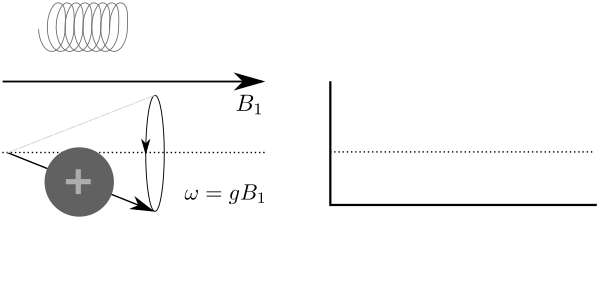
\includegraphics[width=\textwidth]{img/spin0.png}
    \caption{Spin sometido a un campo magn\'etico debil}
    \label{fig:nosignal}
\end{minipage} ~ %add desired spacing between images, e. g. ~, \quad, \qquad, \hfill etc. %(or a blank line to force the subfigure onto a new line) 
\hfill
\begin{minipage}[b]{0.49\textwidth}
    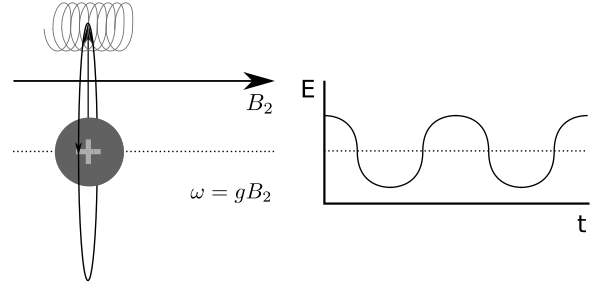
\includegraphics[width=\textwidth]{img/spin1.png}
    \caption{Resultado de aumentar el campo magn\'etico}
    \label{fig:signal}    
\end{minipage} ~ %add desired spacing between images, e. g. ~, \quad, \qquad, \hfill etc. %(or a blank line to force the subfigure onto a new line) 

\end{figure}

\vspace{0.1cm}
Vayamos ahora al plano m\'edico. El cuerpo est\'a compuesto por distintos 
tipos de tejidos, cada uno con su propia composici\'on qu\'imica, lo cual 
determina un momento magn\'etico distinto para cada uno de ellos, y por ende
un tiempo de relajaci\'on particular. Esto implica que al poner a un paciente
dentro de un campo magn\'etico, cada tejido comenzara a generar un momento 
en base a la poblaci\'on de protones que posea. Como ya fue dicho, una forma de
medir el tiempo de relajaci\'on de estos es utilizando un campo magn\'etico. 
El problema es que si uno intentara administrar energ\'ia al sistema simplemente
aumentando la fuerza del campo magn\'etico terminar\'ia da\~nando al paciente. 
Aqu\'i es donde se aprovecha la frecuencia de Larmor. Conociendo la composici\'on
qu\'imica de cada tejido es posible calcular su frecuencia angular. Luego, 
mediante el efecto de resonancia es posible transmitir energ\'ia al sistema
simplemente emitiendo ondas en esa misma frecuencia. \\

\begin{figure}[h!]
                                                                                                                        
\begin{minipage}[b]{0.49\textwidth}
    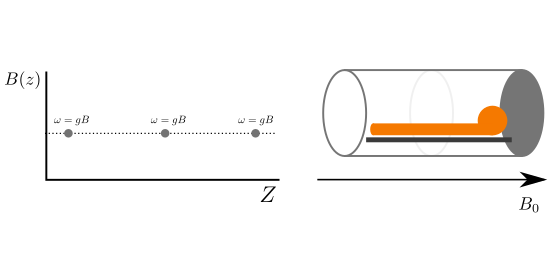
\includegraphics[width=\textwidth]{img/grad0.png}
    \caption{\small  Campo uniforme, todos los protones poseen la misma velocidad angular}
     \label{fig:unif}
\end{minipage} ~
\hfill
\begin{minipage}[b]{0.49\textwidth}
    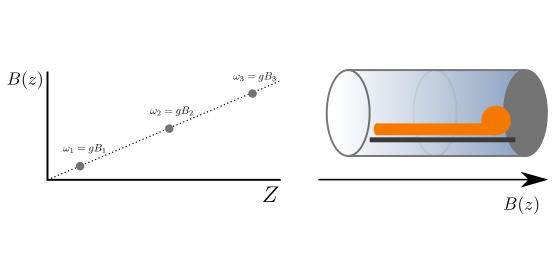
\includegraphics[width=\textwidth]{img/grad1.png}
    \caption{\small Campo gradiente, la velocidad angular de los protones var\'ia linealmente }
    \label{fig:grad}
\end{minipage} ~

\end{figure}  

\vspace{0.1cm}

Los resonadores magn\'eticos son dispositivos con la capacidad de generar 
campos y pulsos en diferentes frecuencias, en partocular todo resonador encendido
est\'a emitiendo constantemente un campo homog\'eneo $B_0$ (ver Figura \ref{fig:unif}). 
El problema entonces es: c\'omo obtener el tiempo de relajaci\'on 
de un punto particular del cuerpo. Para esto es posible utilizar campos 
gradientes. Un campo gradiente es un campo que var\'ia su potencia linealmente
a lo largo de una direcci\'on, provocando que todas los protones a lo 
largo de esa direcci\'on var\'ien su frecuencia angular de manera predecible. 
Aplicando un campo gradiente $G_z$ en la direcci\'on $z$ (ver Figura \ref{fig:grad})
sobre el paciente haremos que la velocidad en funci\'on de la posici\'on sea:
$\omega(z) = B_z(z) g$, esto nos asegurara que si aplicamos el pulso de RF a una
frecuencia de $B_z(z_o) g$, solo los protones que se encuentran en la posici\'on
$z=z_o$ comenzaran a resonar, por lo que estos ser\'an los \'unicos que generen un 
campo transversal. Cabe destacar que como no es posible generar un pulso con
exactamente la frecuencia deseada, tambi\'en resonaran los protones que se 
encuentren cerca, por lo que tendremos un intervalo $[z_o-\epsilon,z_o+\epsilon]$
resonando. A este proceso se lo denomina \textit{slice selection}. Podemos pensar 
el slice como una matriz de dos dimensiones sobre el eje $z$. Si ahora aplicamos
un campo gradiente $G_\psi$ en la direcci'on $y$, suceder\'a que todas las 
filas de nuestra matriz adquiriran diferentes velocidades angulares. Al apagar
$G_\psi$ todos los protones volveran a preceder respecto al campo $B_0$, pero
est\'a vez estaran desfasados por filas (ver Fig. \ref{fig:kspace}). Encendiendo
un tercer campo gradiente $G_\upsilon$ sobre la direcci\'on $x$ conseguiremos
que cada columna posea una frecuencia distinta y cada fila una fase distinta.
Repitiendo este procedimiento varias veces cambiando solo la intensidad de
$G_\psi$ podemos armar lo que se conoce como \textit{k-space}. El \textit{k-space}
es una imagen espacial temporal donde est\'an anotados los valores obtenidos para
cada potencia utilizada, en orden ascendente de potencia. El aplicar una
transformada de Fourier 3D a dicho espacio nos devolver\'a la imagen que
representa el contraste de cada tejido en el \textit{slice} seleccionado. \\

\begin{figure}[h!]
                                                                                                                        
\begin{minipage}[b]{\textwidth}
    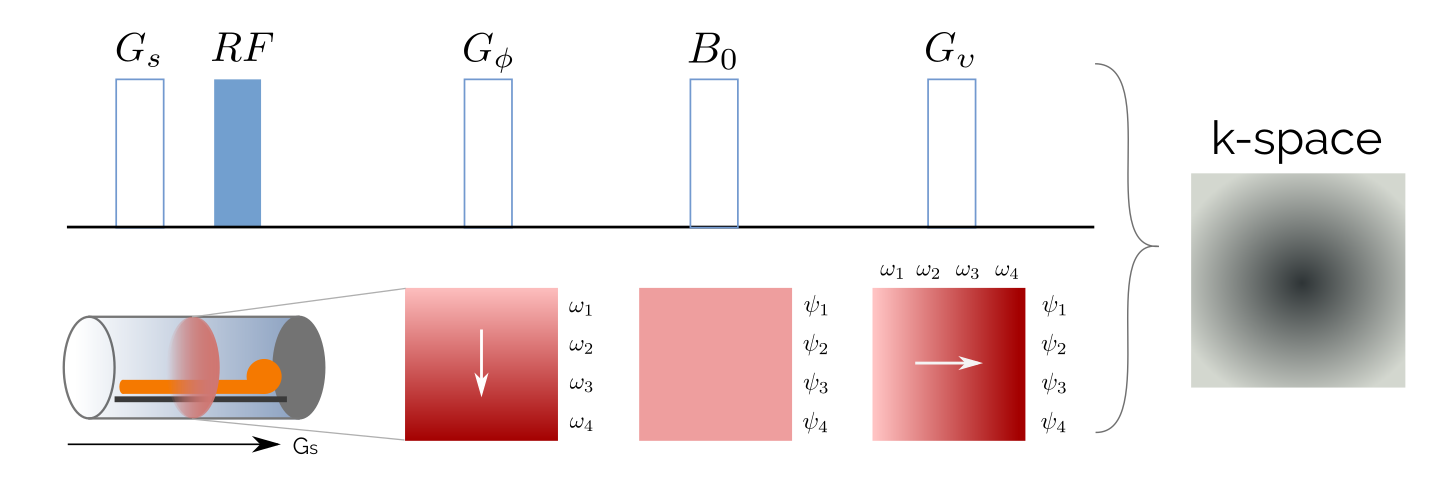
\includegraphics[width=\textwidth]{img/kspace.png}
    \caption{Resumen del proceso de adquisici\'on de im\'agenes en MRI}
    \label{fig:kspace}
\end{minipage} ~

\end{figure}  



\section{Resonancia Magn\'etica de Difusi\'on}

Las mol\'eculas dentro de un fluido en equilibrio no se encuentran est\'aticas,
sino que se mueven realizando un camino aleatorio. A este fen\'omeno se lo 
conoce con el nombre de difusi\'on.  \\

En 1946 Bloch \cite{Bloch1946} prueba que la variaci\'on de la magnetizaci\'on
nuclear en el tiempo se puede expresar como:

$$ \frac{dM(t)}{dt} = \gamma M(t) \times B(t) 
                      - \frac{M(t) \vec{x} + M(t)\vec{y}}{T_2}
                      - \frac{(M(t)-M(0))\vec{z}}{T1} $$

Donde $\gamma$ es la relaci\'on giromagn\'etica, $B$ es la intensidad del campo
magn\'etico y T1, T2 son tiempos de relajaci\'on. Mas tarde, en 1956, H.C. Torrey \cite{Torrey1956}
observa que la magnetizaci\'on tambi\'en se pierde por efecto de la difusi\'on y 
extiende la ecuaci\'on de Bloch:

$$ \frac{dM(t)}{dt} = g M(t) \times B(t) 
                      - \frac{M(t) \vec{x} + M(t)\vec{y}}{T_2}
                      - \frac{(M(t)-M(0))\vec{z}}{T1} 
                      + \nabla \cdot D \nabla M(t) $$

Donde $D$ es el tensor de difusi\'on. Esta relaci\'on se conoce como la
ecuaci\'on de Bloch-Torrey.\\

Imaginemos el siguiente experimento: luego de aplicar el pulso RF agregamos un
campo gradiente $G_1=G_d$ durante un tiempo $\delta$ peque\~no. Como ya explicamos,
esto generar\'a un desfase entre los spines de los protones. El aplicar $G_2=-G_d$
luego de $\Delta$ deber\'ia provocar que los spines se vuelvan a alinear. Sin
embargo, los protones que se encuentren en un fluido estar\'an sometidos al
efecto de la difusi\'on. Esto sucede, por ejemplo, en el interior de los
axones. Dependiendo del tiempo $\delta$ los protones se habr\'an movido cierta
distancia, provocando que el campo magn\'etico los alcance en distintas 
posiciones. Por ende su velocidad angular se ver\'a afectada de manera distinta 
a la esperada si no se hubieran movido. Esto nos indica que si hay difusi\'on
entonces habr\'a un desfase en esa poblaci\'on de neutrones (ver Figura 
\ref{fig:dmri}).\\

\begin{figure}
                                                                                                                        
\begin{minipage}[b]{\textwidth}
    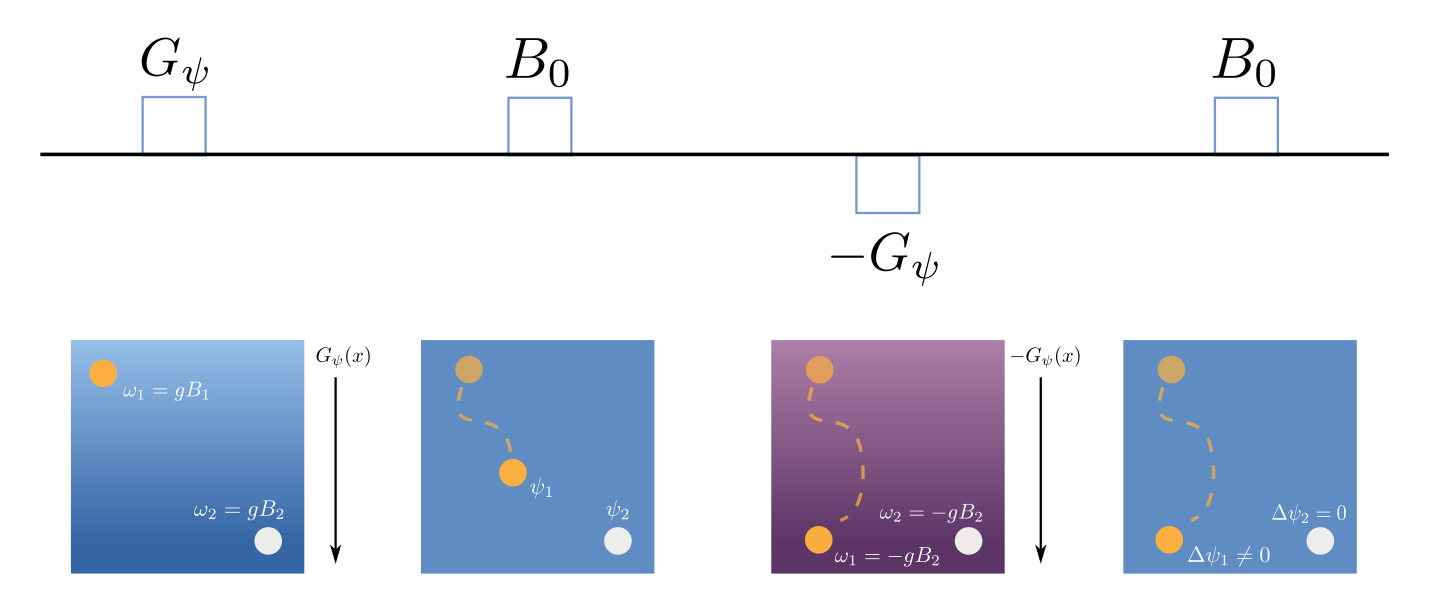
\includegraphics[width=\textwidth]{img/dmri.png}
    \caption{Modificar la secuencia permite medir la intensidad de difusi\'on}
    \label{fig:dmri}
\end{minipage} ~

\end{figure}  

Recordemos que la se\~nal medida en un resonador magn\'etico proviene del 
momento magn\'etico de los protones. Es importante entender que por limitaciones
f\'isicas de los dispositivos es imposible obtener la se\~nal producida por un
solo prot\'on. Lo que se mide es la resultante de los momentos magn\'eticos de 
todos los protones dentro de un espacio. Si todos los protones est\'an precediendo
a la misma velocidad sobre el mismo plano, entonces la resultante m\'axima se
obtiene cuando todos poseen la misma fase. Esto es, todos se encuentran en la
misma posici\'on al mismo tiempo, rotando juntos. Por ende, el desfase producto
de la difusi\'on se traducira en perdida de se\~nal.\\

\begin{wrapfigure}{r}{0.5\textwidth}
    \begin{center}
        \vspace{-1cm}
        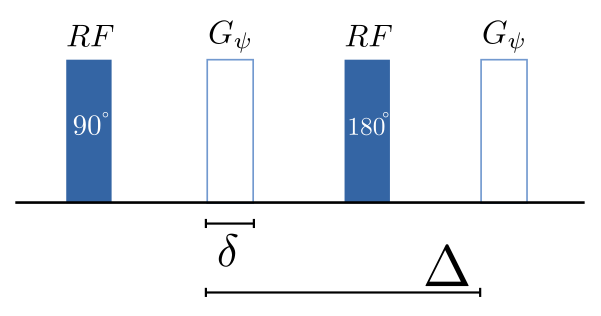
\includegraphics[width=0.4\textwidth]{img/fgp.png}
        \caption{Pulsed Gradient Spin Echo}
        \label{fig:fgp}
    \end{center}
\end{wrapfigure}  

En 1965 Stejskal y Tanner \cite{Stejskal1965} cren una secuencia denominada 
\textit{Pulsed Gradient Spin Echo}. En la misma utilizan dos pulsos de RF y 
un gradiente magn\'etico para generar un desfase entre los protones (ver Figura
\ref{fig:fgp}). Luego demuestran que asumiendo un $\delta$ peque\~no la ecuaci\'on
de Bloch-Torrey tiene soluci\'on, y la atenuaci\'on de la se\~nal se puede expresar
como:

\vspace{0.3cm}

\begin{equation}
    E(g, \delta, \Delta) = 
    \frac{S(g, \delta, \Delta)}{S_0} =
         e^{-\gamma^2 g^2 \delta^2 \left(\Delta - \frac{\delta}{3}\right) D} 
    \label{eq:st}
\end{equation}

\vspace{0.1cm}
  
Donde $E(g, \delta, \Delta)$ es la atenuaci\'on de la se\~nal obtenida; 
$g$ es la intensidad del gradiente magn\'etico; $S_0$ es la se\~nal obtenida sin
utilizar gradientes ($g=0 T/m$); $\gamma$ es la relaci\'on giromagn\'etica del 
prot\'on; $\delta$ es el tiempo que el gradiente est\'a encendido; $\Delta$ es el
tiempo entre las activaciones del gradiente y $D$ representa el coeficiente de
difusi\'on. La raz\'on por la cual se divide la se\~nal obtenida por $S_0$ es
porque la se\~nal en cada punto depende fuertemente de la densidad de protones
que hay en el mismo, si no ponderamos dicha densidad, es imposible comparar la
intensidad de difusi\'on en distintas regiones. \\

En 1985 Le Bihan \cite{LEBIHAN} adapta esta t\'ecnica para medir la difusi\'on 
de las part\'iculas agrupando todos los par\'ametros del experimento dentro de 
un mismo par\'ametro $b$:

$$ b = \gamma^2 g^2 \delta^2 \left(\Delta - \frac{\delta}{3}\right) $$ 

Esto simplifica la ecuaci\'on \ref{eq:st}:  

$$ E(b) = \frac{S(b)}{S_0} = e^{-b D} $$

Donde $b$ representa el reciproco de la intensidad de difusi\'on. \\

En 1994 Basser et al. \cite{Basser1994} proponen medir la atenuaci\'on de se\~nal
en distintas direcciones y luego aproximar el coeficiente de difusi\'on con un 
tensor de segundo orden. Un tensor es una matriz multidimensional asociado a una
base, que posee una ley de transformaci\'on  para indicar  c\'omo cambian los 
componentes del tensor al cambiar de base. Esta t\'ecnica sienta las bases de lo
que se conoce como \textit{Diffusion Tensor Imaging} (DTI). En DTI el tensor 
mas utilizado representa un elipsoide en $R^3$. La matriz que lo representa
es  sim\'etrica, por ello es que se necesitan tomar al menos seis adquisiciones: 

$$
    D =
    \begin{pmatrix}
             D_{xx} & D_{xy} & D_{xz} \\
             D_{xy} & D_{yy} & D_{yz} \\
             D_{xz} & D_{yz} & D_{zz}    
    \end{pmatrix}
$$

\vspace{0.1cm}

El problema con utilizar este es que no permite representar correctamente
el cruce de fibras dentro de cada voxel dado que las caracteriza con un solo
elipsoide.\\

En 1991 Callaghan et al \cite{Callaghan1991} desarrollan el \textit{q-space analysis}.
Esto permite realizar microscop\'ia mediante dMRI. Utilizando el trabajo de Stejskal
y Tanner prueban que es posible obtener la siguiente relaci\'on entre la se\~nal
atenuada y una transformada de Fourier:

$$E(q,\Delta) =  \frac{S(q,\Delta)}{S_0} = \int_{R^2}{p(r;\Delta)e^{-2\pi i q r} dr} $$
$$ q = \frac{\gamma \delta g}{2\pi} $$

Donde $p(r;t)$ es la densidad de probabilidad de que una poblaci\'on de 
part\'iculas se desplace en direcci\'on $r$ durante un tiempo $t$. $p(r;t)$ es
caracter\'istico del compartimiento donde se mueven las part\'iculas. \\

Una de las principales ventajas de \textit{q-space} sobre DTI es que no asume
ning\'un modelo a priori, esto permite definir distintos tipos de modelos para
$p(r,t)$ que caracterizan mejor el cruce de fibras. \textit{Spherical Harmonics}
\cite{Tuch2004} o \textit{Constrained Spherical Deconvolution} \cite{Tournier2004}.
son ejemplos de ello. \\



\chapter{Parcelando la Corteza Cerebral}

En el cap\'itulo anterior presentamos los fundamentos f\'isicos de la Resonancia
Magn\'etica Nuclear y como es posible utilizar estos para caracterizar la 
difusi\'on en el cerebro. Nuestro objetivo ahora es parcelar la corteza cerebral
haciendo uso de un criterio estructural. En particular, utilizando una imagen de
difusi\'on, queremos generar una parcelaci\'on mediante el agrupamiento de
tractogramas. Para ello es necesario primero seleccionar los voxels que ser\'an
utilizados como semilla de cada tractograma; luego generarlos y finalmente 
agruparlos usando alg\'un algoritmo de clustering. Dejamos el siguiente diagrama
para ser utilizado como referencia de los pasos a seguir: \\

\begin{figure}[h!]

\centering
\begin{minipage}[b]{\textwidth}
    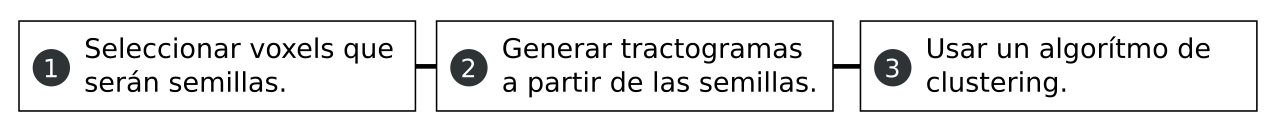
\includegraphics[width=\textwidth]{img/diagrama.png}
    \caption{\small \textit{Pipeline} del proceso de parcelaci\'on }
    \label{fig:diagrama}
\end{minipage} ~

\end{figure}  

\section{Materiales utilizados en el estudio}

Todos nuestros experimentos fueron realizados con sujetos descargados de la base
de datos de \textit{Human Connectome Project}. Las ventajas de utilizar estos
datos son muchas: Tanto la imagen de difusi\'on como la anat\'omica se encuentran
ya preprocesadas \cite{Glasser2013}; cada sujeto posee una parcelaci\'on que, entre
otras cosas, permite separar la materia blanca de la gris; y cada sujeto posee una
superficie que representa su corteza cerebral.\\

\section{Seleccionando voxels que ser\'an semillas}

Como ya dijimos, la materia gris est\'a compuesta principalmente por neuronas,
y la materia blanca por axones que las comunican. Como cada neurona
posee asociado un ax\'on, colocar semillas en la interfaz entre la materia gris
y la blanca permite caracterizar las neuronas de la corteza \cite{Mori2002}
\cite{Anwander2006}. Cibu et al. \cite{Thomas2014} muestran que la materia blanca
cercana a la materia gris est\'a interconectada por peque\~nos axones. Como
estamos interesados en realizar un estudio de las conexiones entre regiones
distantes del cerebro, decidimos situar las semillas a \textit{3mm} de la corteza,
evitando as\'i el efecto de \'estos axones locales. El problema es que la corteza
del cerebro no es uniforme, sino que est\'a llena de surcos y circunvoluciones. 
Calcular la distancia entonces no es inmediato, necesita un m\'etodo que tome
estas propiedades en cuenta. A continuaci\'on presentamos el m\'etodo
\textit{Fast Marching Method} y como es posible utilizarlo para posicionar las
semillas respetando la forma de la materia blanca. \\

\textit{Fast Marching Method} es un m\'etodo para resolver num\'ericamente una
versi\'on restringida de la ecuaci\'on \textit{Eikonal}. La misma, en su forma
general, es una ecuaci\'on diferencial no lineal que se encuentra com\'unmente 
en problemas de propagaci\'on de onda. Tiene la forma: 

$$ V(x) | \nabla u(x) | = F(x) , x \in \Omega $$ 

Donde $\Omega$ es un subconjunto abierto de $R^n$ con un
\textit{buen comportamiento} en su borde. $F(x)$ se denomina el costo temporal y
$V(x)$ es la velocidad de la onda en cada punto. En el caso particular que
queremos resolver $u(x_\omega) = 0, x \in \delta\Omega$;  $F(x)=1$ y $V(x)=1$,
por lo que la ecuaci\'on se resume a:

$$ | \nabla u(x) | = 1 , x \in \Omega $$ 

$u(v)$ en este caso representa el tiempo que tarda la onda en llegar desde
alg\'un elemento del borde hasta el punto $v$ movi\'endose a velocidad constante
de una unidad de espacio por unidad de tiempo. Dada la forma de la velocidad, 
$u(v)$ tambi\'en representa \textbf{la distancia mas corta que existe entre cualquier
punto $v$ de la imagen y el borde de $\Omega$}. Dependiendo la orientaci\'on que 
se elija, las distancias a los puntos internos de la superficie ser\'an negativas
y las distancias a los puntos externos positivas (Figura \ref{fig:fmm}). 
\textit{FMM} resuelve este problema en tiempo $O(n log(n))$ \cite{Sethian2001},
siendo $n$ la cantidad de voxels de la imagen.\\

\begin{figure}[h!]

\centering
\begin{minipage}[b]{0.7\textwidth}
    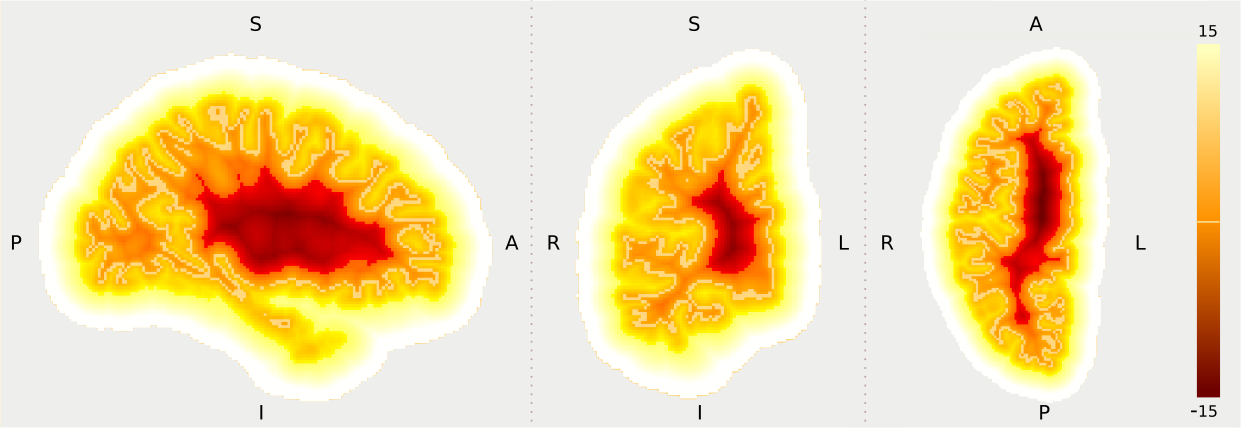
\includegraphics[width=\textwidth]{img/fmm.png}
    \caption{\small FMM sobre el hemisferio derecho, el borde la materia blanca fue
    resaltado intensionalmente}
    \label{fig:fmm}
\end{minipage} ~

\end{figure}  

Es posible utilizar este algoritmo para seleccionar voxels a cierta profundidad
en la materia blanca. Usando como borde la corteza cerebral podemos crear un mapa
de distancias en la materia blanca. El gradiente de este mapa de distancias es un
campo vectorial donde cada vector apunta hacia el interior de la materia blanca.
Caminar partiendo desde los puntos en la siguiendo este campo permite adentrarse 
respetando la morfolog\'ia de la materia blanca. Una ventaja de este m\'etodo es
que permite guardar un mapeo entre cada coordenada de la superficie y la semilla
que la representa. Otra ventaja es que es posible realizar todo el proceso en tiempo
$O(n log(n))$. \\


\section{Estabilidad algor\'itmica}
\label{sec:estabilidad}

Un tractograma es una imagen donde cada voxel representa la probabilidad de que
ese punto del cerebro est\'e conectado a la semilla elegida mediante un conjunto
de axones. Una forma de crear el tractograma de una semilla es generar un gran
n\'umero de streamlines desde ella y luego calcular la frecuencia de visitas por
cada voxel. Se denomina \textit{streamline} al camino que puede realizar una
part\'icula de agua siguiendo un mapa probabil\'istico de transiciones entre voxels.
Es importante destacar que el estimar los tractogramas de esta manera genera un 
sesgo respecto a la distancia. Cuanto m\'as lejos est\'a un voxel mayor es el 
n\'umero de transiciones probabil\'isticas necesarias para llegar a \'el. \\

Dipy es una librer\'ia para python que contiene, entre otras herramientas,
varios algoritmos para generar \textit{streamlines}. Para este trabajo elegimos
utilizar la implementaci\'on de \textit{LocalTracking} (LT de aqu\'i en mas) que
se encuentra en el paquete \textit{dipy.tracking.local}; y una implementaci\'on 
propia (MSL de aqu\'i en m\'as). Ambos algoritmos poseen una estructura 
similar: Encuadran la imagen de difusi\'on en un modelo; crean un objeto que les
permita seleccionar una direcci\'on hacia donde caminar en base a la posici\'on
actual y se mueven hasta cumplir un criterio de parada.\\

En ambos casos modelamos la informaci\'on de dMRI usando el \textit{Constrained
Spherical Deconvolve Model}. La principal diferencia entre los algoritmos surge
en la forma en que seleccionan c\'omo avanzar. Dado el conjunto de direcciones 
iniciales, esto es, las direcciones posibles a tomar desde la semilla,
LT intenta en sucesivas repeticiones del experimento elegir una distinta, 
usando as\'i todas al menos una vez. MSL por otro lado selecciona una al
azar cada vez que repite el experimento. A su vez, LT utiliza un criterio de 
parada basado en la anisotrop\'ia de la difusi\'on; MSL usa una mascara ya 
predefinida. Para mayores detalles referirse al Anexo\\

Algunas preguntas interesantes a realizar sobre los tractogramas son: ¿Al repetir
el experimento, podremos obtener el mismo tractograma?; ¿Cu\'antas part\'iculas son
necesarias para ello? y ¿Qu\'e tanto difieren los resultados entre los distintos 
algoritmos de tractograf\'ia?\\

Para determinar si los algoritmos se estabilizaban y el n\'umero de part\'iculas
necesario para que eso suceda utilizamos la t\'ecnica estad\'istica de
\textit{bootstrap} \cite{Efron1982}. Bootstrap es una forma de aproximar la
distribuci\'on del muestreo de un estad\'istico en base a calcular el mismo
utilizando sucesivos remuestreos de los datos con repeticiones. Esto es
especialmente \'util cuando el n\'umero de muestras que se posee de la poblaci\'on
no es significativamente alto. En nuestro caso situamos mas de setecientas
semillas en el \'Area de Broca y luego generamos quince mil streamlines por cada
una. Luego calculamos el tractograma medio y la varianza de cada voxel utilizando
mil submuestras aleatorias del mismo tama\~no. Esto se repiti\'o con varios
tama\~nos de submuestra para estudiar as\'i la variabilidad a medida que la
cantidad de part\'iculas crec\'ia.\\


\section{Clustering de semillas: Moreno-Dominguez.}

Moreno-Dominguez et al. \cite{Moreno-Dominguez2014} implementan el algoritmo
\textit{Agglomerative Hierarchical Clustering} para agrupar los tractogramas. 
En este algoritmo, cada \textit{feature} comienza en un cluster distinto. Luego,
el algoritmo selecciona iterativamente dos clusters siguiendo alg\'un criterio
de similitud; los agrupa en un nuevo cluster y crea un elemento representativo
de este. La jerarqu\'ia resultante de agrupar todos los clusters es expresada
como un dendrograma. En el trabajo de Moreno-Dominguez utilizan como medida de
similitud la distancia coseno (Ecuaci\'on \ref{eq:cosine}) y como criterio de
\textit{linkage} el centroide (Ecuaci\'on \ref{eq:centroide}).

\begin{figure}[h!]
                                                                                                                        
\begin{minipage}[b]{0.49\textwidth}
    \begin{equation}
        \label{eq:cosine}
        simil_{cos}(X,Y) = 1 - \frac{ X \cdot Y }{||X|| ||Y||}
    \end{equation}
\end{minipage} ~
\hfill
\begin{minipage}[b]{0.49\textwidth}
    \begin{equation}
        \label{eq:centroide}
        centroide(X,Y) = \frac{ n_X X + n_Y Y}{n_X + n_Y}
    \end{equation}
    %\caption{\small $X, Y \in R^m; n_Z = #Z$}
\end{minipage} ~

\centering
\vspace{0.5cm}
\small{$X, Y \in R^m$, $n_z = \#z$}

\end{figure}  

Para mejorar los resultados del \textit{clustering} realizan distintos tipos de
preprocesamiento en varias etapas. Aqu\'i daremos solo una breve descripci\'on 
de los mas relevantes, para mayores detalles favor de referirse al paper. \\

Una de las primeras modificaciones es al algoritmo 
\textit{Agglomerative Hierarchical Clustering}. Dado un n\'umero $k$,
las primeras $k$ iteraciones son entre clusters vecinos y de tama\~no similar.
Esto es, solo los clusters que se encuentran a menos de cierta distancia f\'isica
en el cerebro pueden ser unidos. A su vez, solo se unen los clusters que poseen
un tama\~no similar para que el dendrograma crezca de manera balanceada. \\


\settowidth\mylen{procedure Clustering(}
\addtolength\mylen{\parindent}

\begin{algorithm}[h]
\caption{Modificaciones al algoritmo Agglomerative Hierarchical Clustering.}
\label{alg:morenoahc}
\begin{algorithmic}[1]

\Procedure{Clustering(k\_pasos: primeros K pasos, \\ \hspace*{\mylen}
                      tractogramas: mat. de tractogramas, \\ \hspace*{\mylen}
                      vecinos: mat. de vecinos, \\ \hspace*{\mylen}
                      distancias: mat. de distancia clusters ) }{}
                      
    \State \emph{jerarquia} $\gets \emptyset$
                      
\For{\emph{k} in [1, cant(\emph{tractogramas})] }

    \If{\emph{k} $>$ \emph{k\_pasos}}

        \State \emph{$C_x$, $C_y$} $\gets$ clusters tales que $x$ e $y$ poseen \emph{distancia} minima      
            
    \Else{}

        \State \emph{$C_x$, $C_y$} $\gets$ $x$ e $y$ son \emph{vecinos}; 
                                   de \emph{distancia} minima y de tama\~no similar.

    \EndIf
    
    \State {tractogramas} $\gets$ eliminar clusters $C_x$, $C_y$

    \State {centroide} $\gets$ computar explicitamente el centroide $(C_x,C_y)$ 

    \State {tractogramas} $\gets$ agregar \emph{centroide}
    
    \State \emph{jerarquia} $\gets$ agregar la union $(C_x,C_y)$
    
    \For{ $C_z$ in \emph{tractogramas} }
        \State \emph{D} $\gets$ computar explicitamente distancia coseno de $C_z$ al \emph{centroide}
        \State \emph{distancias} $\gets$ actualizar distancia entre $(C_x,C_y)$ y \emph{centroide} con \emph{D}
    \EndFor            
    
\EndFor

\State \Return \emph{jerarquia} 
 
\EndProcedure 

\end{algorithmic}
\end{algorithm}

\vspace{1cm}

Una vez obtenido el dendrograma proceden a eliminar las inversiones dentro del
mismo. Una inversi\'on sucede cuando se unen dos clusters con una distancia 
interna mayor a la distancia entre ellos. Las inversiones no cambian la 
jerarqu\'ia de los clusters, sino que solo complican la interpretaci\'on visual
de los datos \cite{Murtagh1985}. Una forma de eliminarlas es colapsando las 
ramas que la componen en una sola jerarqu\'ia con mas de dos elementos. Un 
ejemplo de inversi\'on y el resultado de quitarla se muestran en las Figuras 
\ref{fig:inversion} y \ref{fig:no_inversion} respectivamente. 


\begin{figure}[h!]
                                                                                                                        
\begin{minipage}[b]{0.49\textwidth}
    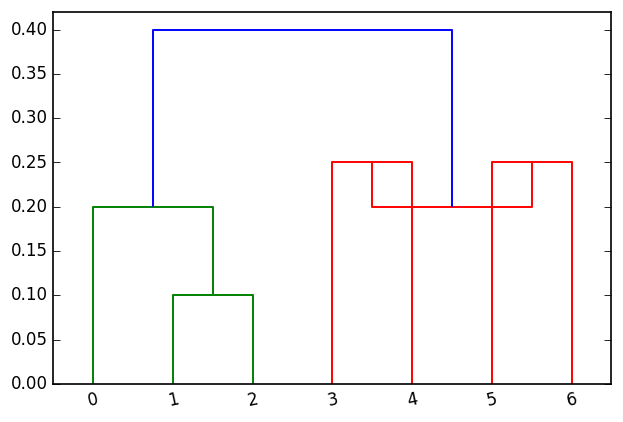
\includegraphics[width=\textwidth]{img/inversion_0.png}
    \caption{\small Dendrograma de inversi\'on.}
     \label{fig:inversion}
\end{minipage} ~
\hfill
\begin{minipage}[b]{0.49\textwidth}
    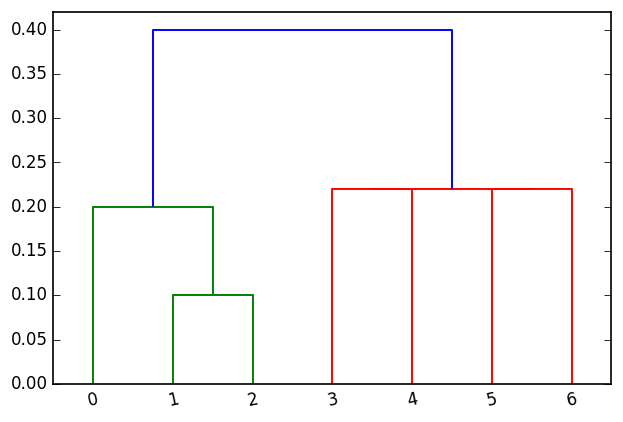
\includegraphics[width=\textwidth]{img/inversion_1.png}
    \caption{\small Dendrograma con inversi\'on corregida. }
    \label{fig:no_inversion}
\end{minipage} ~

\end{figure}  

\vspace{0.1cm}

Otro paso de preprocesamiento es el quitar \textit{outliers} del dendrograma.
Esto en realidad lo hacen durante la etapa de \textit{clustering}. Evitan que los
clusters de un solo elemento se unan a otros clusters si la (di)similitud es 
mayor a cierto \textit{threshold}. Al hacer este paso durante el \textit{clustering}
previenen que los \textit{ouliers} afecten la forma de los nuevos centroides.\\

Una vez finalizados todos los pasos el resultado es un dendrograma. Para parcelar
la corteza solo es necesario seleccionar una altura en la cual cortar dicho
dendrograma. Los clusters que est\'en por debajo de ese corte ser\'an las distintas
parcelas. \\




\chapter{Contribuciones}

En el cap\'itulo anterior presentamos c\'omo generar los tractogramas y el 
estado del arte para agruparlos. En este cap\'itulo presentamos las contribuciones
de nuestro trabajo. Comenzamos con una contribuci\'on menor que es estudiar la 
estabilidad del algoritmo de tractograf\'ia utilizado en el trabajo. Luego hacemos
un an\'alisis te\'orico del estado del arte y mostramos algunas de las 
problem\'aticas que posee. Finalmente utilizamos una funci\'on para transformar
los tractogramas al espacio eucl\'ideo y mostramos como esto permite mejorar tanto
la complejidad espacial como temporal del algoritmo de \textit{clustering}. \\

\section{Estudio de la convergencia de los tractogramas}
\label{sec:convergencia}

El diagrama de la figura \ref{fig:diagrama} divide el proceso de 
parcelaci\'on de la corteza en varios pasos. El tercero de ellos consiste
en generar tractogramas. Un tractograma para una semilla $s$ es una imagen
donde cada voxel $v$ representa la probabilidad de que $v$ est\'e 
conectado a $s$ mediante un conjunto de axones. En la secci\'on 
\ref{sec:tractogramas} presentamos una forma de crear tractogramas
mediante un procedimiento Monte Carlo generando \textit{streamlines}. Un
\textit{streamline} representa el movimiento aleatorio de una part\'icula
de agua dentro de la materia blanca. Los tractogramas creados de esta
manera son inherentemente estoc\'asticos. Esto genera algunas preguntas
interesantes: ¿Al repetir el experimento, podremos obtener el mismo
tractograma? y ¿Cu\'antas part\'iculas son necesarias para ello?. Para
contestar estas preguntas utilizamos la t\'ecnica estad\'istica de 
\textit{bootstrap} \cite{Efron1982}. \\

\settowidth\mylen{procedure2 tractograma(}
\addtolength\mylen{\parindent}

\begin{algorithm}[h!]
\caption{Algoritmo de tractograf\'ia utilizado}\label{alg:localtracking}
\begin{algorithmic}[1]

\Procedure{tractograma(anatomica: img. anat\'omica, \\ \hspace*{\mylen}
                              dMRI: img. de difusi\'on, \\ \hspace*{\mylen}
                              S: semilla, P: num. part\'iculas)}{}

\State \emph{csd} $\gets$ Constrained Spherical Deconvolution Model of \emph{dMRI}. 

\State \emph{mapa\_probabilistico} $\gets$ Mapa desde los coeficientes
                                           Spherical Harmonics en \emph{csd}

\State \emph{mapa\_visitas} $\gets$ matriz nula con mismas dimensiones que la anat\'omica

\For {p in [1$\dots$P]}

    \State $streamline_p$ $\gets \emptyset$
    \State \emph{posicion\_actual} $\gets$ posicion de S
    
    \While {posicion\_actual en materia blanca}

        \State \emph{direccion\_actual} $\gets$ elegir direccion desde
                                               \emph{mapa\_probabilistico} 
        
        \State \emph{posicion\_actual} $\gets$ avanzar solo un voxel en
                                               \emph{direccion\_actual} 
        
        \State $streamline_p$ $\gets$ agregar \emph{posicion\_actual}    
        
    \EndWhile
    
    \For {\emph{pos} in $streamline_p$}
        \State \emph{mapa\_visitas[pos]} $\gets$ \emph{mapa\_visitas[pos]} + 1
    \EndFor
    
\EndFor

\State \emph{tractograma} $\gets$
                                 \emph{log(mapa\_visitas+1)} / log(P+1)    

\State \Return \emph{tractograma} 
 
\EndProcedure

\end{algorithmic}
\label{alg:itract}
\end{algorithm}

\vspace{0.3cm}

\textit{Bootstrap} permite estimar la distribuci\'on de un estad\'istico
en base a calcularlo sobre remuestreos con repeticiones de una 
poblaci\'on. El m\'etodo es especialmente \'util cuando el n\'umero de
muestras que se posee no es significativamente alto. Nosotros queremos
estimar la distribuci\'on de la media de los \textit{tractogramas} en 
funci\'on de la cantidad de \textit{streamlines}. En la literatura
se usan hasta $100000$ \textit{streamlines} por cada semilla 
\cite{Anwander2006}. \textit{Bootstrap} nos permite realizar este estudio
con muchas menos. \\

Para entender mejor la relaci\'on entre \textit{streamlines} y
tractogramas presentamos en el algoritmo \ref{alg:itract} el pseudoc\'odigo
de la implementaci\'on de tractograf\'ia utilizada. Dicho algoritmo es una
instanciaci\'on del presentado en la secci\'on \ref{sec:tractogramas}. La
imagen de difusi\'on se enmarca en el modelo \textit{Constrained Spherical
Deconvolution} usando la forma propuesta por Aganj et al. 
\cite{Aganj2010}; el mapa de transiciones probabil\'isticas se recupera
usando \textit{Spherical Harmonics} \cite{Descoteaux2007} y el tractograma
se calcula usando la ecuaci\'on \ref{eq:normalizacion} propuesta en el 
trabajo de Moreno-Dominguez et al. \cite{Moreno-Dominguez2014}. \\

\begin{algorithm}
\caption{Procedimiento de \textit{Bootstraping}}\label{alg:localtracking}
\begin{algorithmic}[1]

\Procedure{estabilidad(S: semilla)}{}

\State \emph{streamlines} $\gets$ $\emptyset$

\Loop{ 15000 veces }
    \State \emph{stream} $\gets$ crear streamline desde S 
    \State \emph{streamlines} $\gets$ agregar \emph{stream}
\EndLoop

\State \emph{medias} $\gets$ $\emptyset$
\State \emph{varianzas} $\gets$ $\emptyset$

\For{\emph{ss\_size} in [200, 500, 800, $\dots$]}

    \State \emph{subsample} $\gets$ $\emptyset$

    \Loop{ 10000 veces }
        \State \emph{tractograma} $\gets$ tomar \emph{ss\_size} streams de
                                          \emph{streamlines} y crear
                                          tractograma
        \State \emph{subsample} $\gets$ agregar \emph{tractograma} 
    \EndLoop
    
    \State \emph{medias} $\gets$ agregar tractograma medio de 
                                 \emph{subsample}
    \State \emph{varianzas} $\gets$ agregar tractograma varianza de 
                                    \emph{subsample}
\EndFor

\State \Return \emph{medias}, \emph{varianzas} 
 
\EndProcedure

\end{algorithmic}
\label{alg:bootstrap}
\end{algorithm}

Usando el algoritmo \ref{alg:itract} generamos $15000$ 
\textit{streamlines} para distintas semillas en el \'area de Broca. Luego
calculamos el tractograma medio y la varianza de cada voxel utilizando
$10000$ submuestras aleatorias del mismo tama\~no. Repetimos esto con
varios tama\~nos de submuestra para estudiar la variabilidad del 
estad\'istico. Este procedimiento se puede ver en el algoritmo 
\ref{alg:bootstrap}.\\

Crear los tractogramas es uno de los pasos necesarios para parcelar la
corteza. Por la forma en que est\'an definidos, los tractogramas son
inherentemente estoc\'asticos. El m\'etodo aqu\'i presentado nos permite
estudiar la estabilidad del algoritmo de tractograf\'ia implementado. De
esta manera podemos comprobar si dado un n\'umero suficiente de 
part\'iculas los tractogramas de una semilla convergen a un mismo 
resultado. \\


\section{An\'alisis del m\'etodo Moreno-Dominguez}

Utilizar \textit{Hierarchical Agglomerative Clustering} con la distancia 
coseno y el \textit{linkage} centroide presenta al menos dos desventajas. 
Primero, la distancia coseno obliga a tener que comparar expl\'icitamente cada
centroide con los clusters existentes. Notemos que esto implica mantener los
clusters en memoria. Por otro lado, el promedio de probabilidades no
necesariamente representa una probabilidad \cite{Pohl2007}. Esto quiere decir
que el centroide de un grupo de tractogramas no necesariamente representa un
tractograma. \\

\subsection{Clustering de vectores colineales}

\begin{figure}[h!]
        \centering
        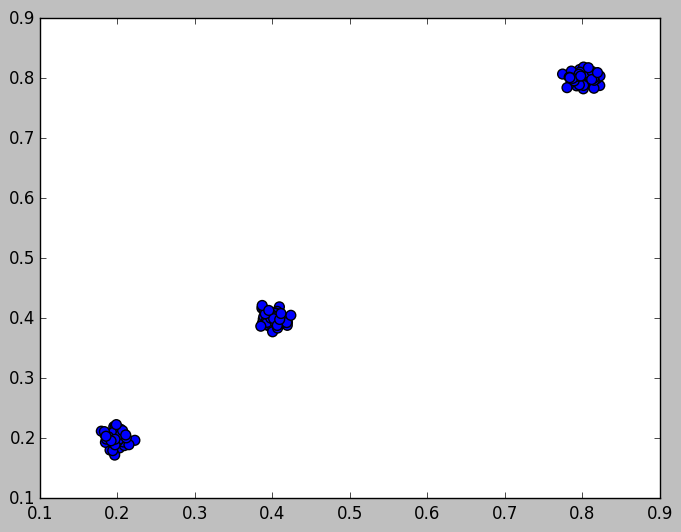
\includegraphics[width=0.5\textwidth]{img/3pop.png}
        \caption{Tres cluster colineales\-}
        \label{fig:3clusters}
\end{figure}

La distancia coseno es una forma de medir co\-rrelaci\'on entre vectores. Por ello,
cuando lo que se intenta agrupar son vectores colineales el resultado es aleatorio.
Por ejemplo, cuando se aplica el procedimiento sobre los puntos de la Figura
\ref{fig:3clusters} el resultado del clustering es la Figura \ref{fig:3moreno}.
Usando LogOdds y la m\'etrica euclidiana se consigue el \textit{clustering} de 
la Figura \ref{fig:3logit}.\\

\begin{figure}[h!]

\centering                                                                                                          
\begin{minipage}[b]{0.85\textwidth}
    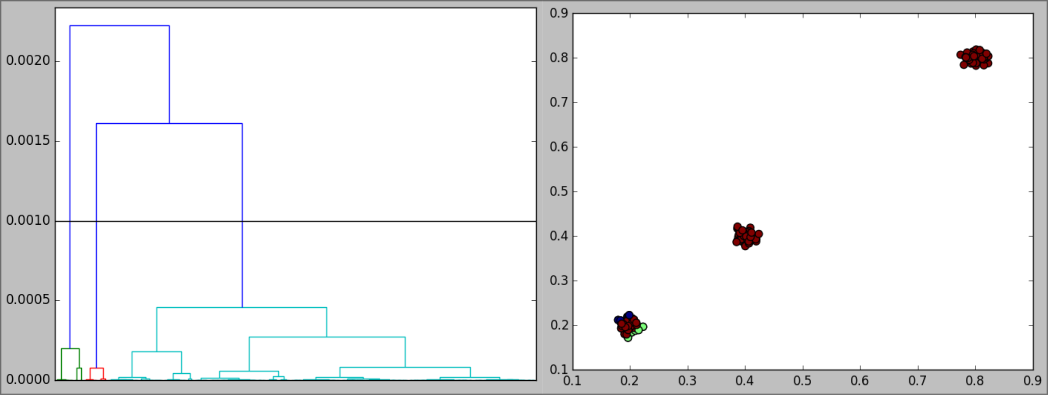
\includegraphics[width=\textwidth]{img/3pop_moreno.png}
    \caption{Clustering resultado de utilizar el m\'etodo Moreno}
    \label{fig:3moreno}
\end{minipage} ~

\end{figure}  

Los tractogramas son im\'agenes que por su naturaleza tienen muchos voxels con 
valores peque\~nos. La Figura \ref{fig:hist_tract} muestra el histograma de los
valores en los tractogramas del \'Area de Broca. Esta gran cantidad
de voxels con valores tan bajos podr\'ia generar ruido en las correlaciones.  

\begin{figure}[h!]
              \centering                                                                                                          
\begin{minipage}[b]{0.8\textwidth}
    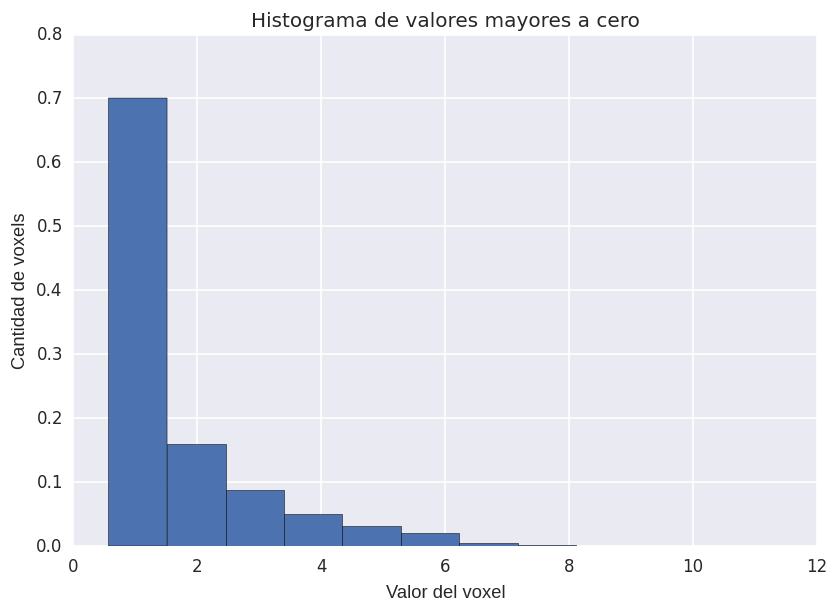
\includegraphics[width=\textwidth]{img/hist_tract.png}
    \caption{Histograma normalizado de los valores en los tractogramas del \'Area de Broca}
    \label{fig:hist_tract}
\end{minipage} ~

\end{figure}  


\subsection{Relaci\'on m\'etrica-\textit{linkage}}

La Figura \ref{fig:cos_cen} muestra cuatro vectores, sus posiciones en coordenadas
polares son: $ p_1 = (0.4, 45^\circ)$;  $p_2 = (0.3, 25^\circ)$;  $p_3 = (0.4, 66^\circ)$
y $p_4 = (0.4, 4.5^\circ) $ \\

Podemos apreciar que al principio $d(p_2,p_3) < d(p_3,p_4) < d(p_1,p_2)$, siendo
$d(x,y)$ la distancia coseno. Sin embargo, luego de utilizar el 
\textit{linkage centroid} sucede que $d(p_1,p_c) < d(p_4,p_c)$. $p_4$
es ahora el punto que mas lejos est\'a del centroide. Creando un representante
$p_m$ usando el \'angulo medio entre $p_2$ y $p_3$ esto no sucede. Este fen\'omeno
se da porque la distancia coseno tiene en cuenta el \'angulo pero el centroide
no. Por lo tanto el centroide no caracteriza al punto medio respecto a la
distancia coseno.\\

\begin{figure}[h!]
                                                                                                                        
\begin{minipage}[b]{\textwidth}
    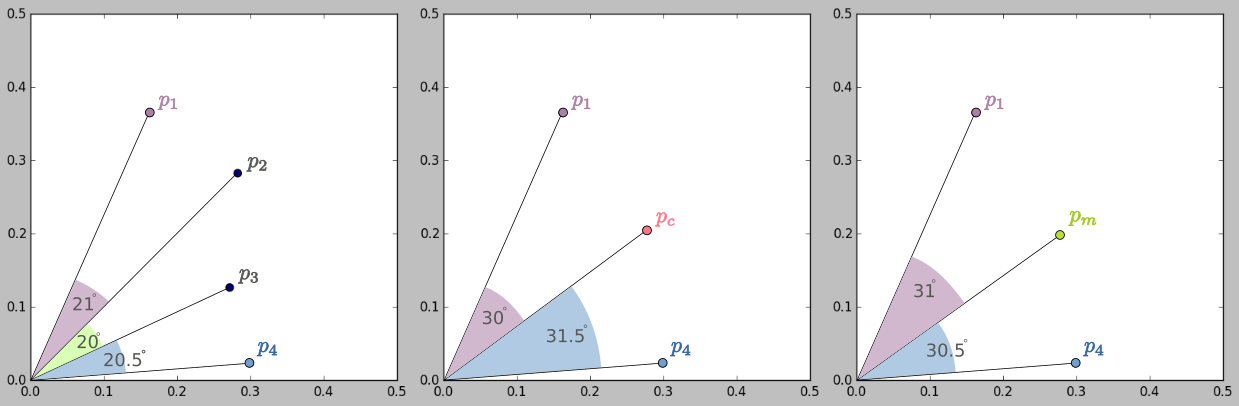
\includegraphics[width=\textwidth]{img/cosine_centroid.png}
    \caption{El centroide no representa el punto medio respecto al \'angulo}
    \label{fig:cos_cen}
\end{minipage} ~

\end{figure}  

\subsection{Complejidad algor\'itmica del clustering}

En todo el proceso el paso mas caro en t\'erminos computacionales es el
\textit{clustering}. En cada iteraci\'on del algoritmo es necesario comparar 
expl\'icitamente cada nuevo centroide con todo el resto de los clusters. Esto 
es costoso computacionalmente. Por cada iteraci\'on es necesario hacer $O(c^2 m)$
operaciones para recalcular todas las distancias, donde $c$ es la cantidad de
clusters y $m$ es la longitud de los mismos. Dadas $n$ semillas iniciales, la 
cantidad de iteraciones a realizar son $n-1$. La complejidad de este m\'etodo es
$O(n^3 m)$.



\section{Clustering en el Espacio Eucl\'ideo}

En la secci\'on anterior presentamos algunos de los inconvenientes te\'oricos 
del m\'etodo propuesto por Moreno-Dominguez. A continuaci\'on mostramos como 
solucionar todos ellos haciendo uso de la tranformaci\'on \textit{logit}. \\

\subsection{Transformaci\'on Logit}

Sea $P_M$ el espacio de una distribuci\'on discreta para $M$ etiquetas: 

$$P_M = \left\{  p | p = (p_1,\dots p_n) \in (0,1)^M , \sum{p_i} = 1 \right\}$$

La funci\'on \textit{logit}:$P_M \rightarrow R^{M-1}$ define una transformaci\'on
entre el espacio $P_M$ y el espacio eucl\'ideo $R^{M-1}$. Dados los vectores $Q \in P^M$ y
$S \in R^{M-1}$:

$$S_i = logit(Q_i) = log\left(\frac{Q_i}{Q_M}\right)$$

Para el caso de $M=2$ permite transformar la distribuci\'on Bernoulli
discreta al espacio eucl\'idio. Podemos ver en la ecuaci\'on \ref{eq:logit} su
expresi\'on anal\'itica y en la Figura \ref{fig:dominio} representaci\'on 
gr\'afica.

\begin{figure}[h!]

\begin{minipage}[b]{0.45\textwidth}

    \begin{equation}
    \vspace{2.85cm}
        \label{eq:logit}
    logit(p) = log\left(\frac{p}{1-p}\right)
    \end{equation}
\end{minipage} ~
\hfill
\begin{minipage}[b]{0.45\textwidth}
    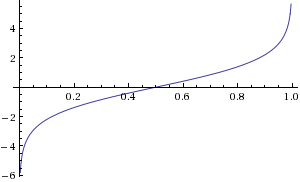
\includegraphics[width=\textwidth]{img/logit.png}
    \caption{Representaci\'on gr\'afica de la funci\'on logit}
    \label{fig:dominio}
\end{minipage} ~

\end{figure}  

Trabajar en el espacio eucl\'ideo nos asegura que la suma y la multiplicaci\'on
por escalares est\'an contenidos en el mismo espacio. Pohl et al. \cite{Pohl2007} 
utilizan esta propiedad para realizar operaciones lineales sobre mapas
probabil\'isticos. A su vez, demuestran que la suma y multiplicaci\'on
por escalares en el espacio eucl\'ideo poseen un significado en el espacio de la
distribuci\'on. \\

\subsection{Modificando el Algoritmo de Clustering}

Asumiendo que cada voxel $v$ de un tractograma proviene de la variable 
aleatoria binaria:

 $$X_v= \textrm{``La semilla est\'a conectada con el voxel v''}$$
 
Es posible transformar el tractograma aplicando la funci\'on \textit{logit} en
cada uno de sus voxels. El resultado es un vector donde cada coordenada se 
encuentra en el espacio eucl\'ideo.  M\'as a\'un, las operaciones lineales entre
los mismos voxels en distintos tractogramas est\'an definidas. Esto nos permite
usar la m\'etrica eucl\'ideana como funci\'on de similitud en \textit{Agglomerative
Hierarchical Clustering}. \\

Transformar de espacio los tractogramas y cambiar la funci\'on de similitud 
posee varias ventajas. Para empezar permite agrupar correctamente vectores
colineales. La Figura \ref{fig:3logit} muestra el resultado de aplicar este
m\'etodo a los vectores de la Figura \ref{fig:3clusters}.  Podemos apreciar 
que las tres poblaciones se encuentran correctamente separadas y bien definidas.\\

\begin{figure}[h!]

\centering
\begin{minipage}[b]{0.85\textwidth}
    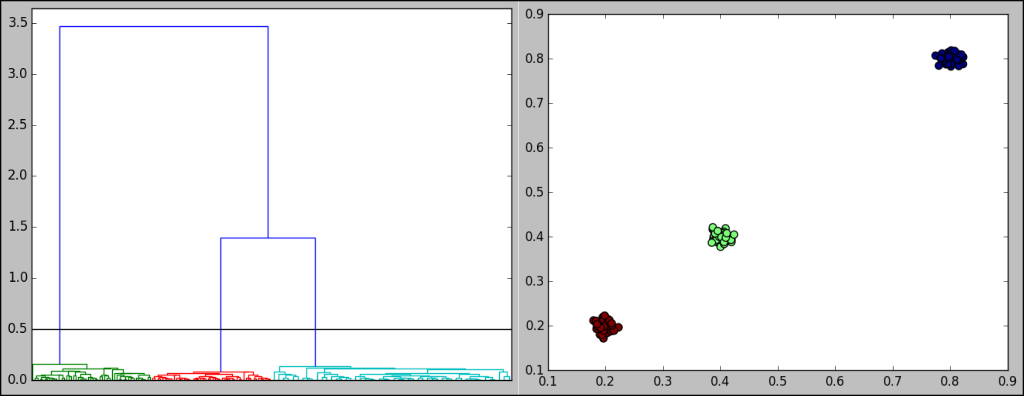
\includegraphics[width=\textwidth]{img/3pop_logit.png}
    \caption{Clustering resultado de utilizar el m\'etodo logit}
    \label{fig:3logit}
\end{minipage} ~

\end{figure}  

Otra ventaja es la buena relaci\'on m\'etrica-\textit{linkage}. Por definici\'on
el centroide es el centro de masa de los clusters. Esto quiere decir que es el 
punto que minimiza la distancia euclidiana entre los clusters que lo componen. 
Por ende, el centroide caracteriza bien el punto medio de los vectores en el
espacio eucl\'ideo. \\

Finalmente, nuestro m\'etodo tambi\'en permite mejorar la complejidad algor\'itmica.
Como ya explicamos, por cada iteraci\'on del algoritmo 
\textit{Agglomerative Herarchical Clustering} es necesario calcular un representante
de la uni\'on y luego computar su distancia al resto. Sin embargo, al usar la
m\'etrica euclideana junto con el \textit{linkage} centroide es posible simplificar
este paso. La formula de Lance y Williams permite computar las nuevas distancias
sin comparar expl\'icitamente los clusters. Esto baja significativamente la
complejidad. Cada iteraci\'on pasa a costar $O(c^2)$ en vez de $O(c^2 m)$, siendo
$c$ la cantidad de clusters y $m$ la longitud de los mismos. Dadas $n$ semillas 
iniciales, la complejidad temporal total del \textit{clustering} es $O(n^3)$. 
Con la distancia coseno era $O(n^3 m)$, siendo $m$ la longitud de los tractogramas.
Recordemos que en el contexto que estamos utilizando este algoritmo $m>>n$. Por
lo tanto, este resultado implica una gran mejora en la eficiencia del algoritmo.  


\subsection{Mejorando la Complejidad Espacial: Matrices Ralas}

Durante la etapa de \textit{clustering} es conveniente tener todos los
tractogramas en memoria. En nuestro caso, la matriz con los \textbf{tractogramas
sin transformar} del \'Area de Broca tiene dimensiones $762\times3587328$. 
Asumiendo que cada valor se representa usando $8$ Bytes, esta matriz ocupa un 
total de aproximadamente $20$ Gigabytes. Sin embargo, solo un $1\%$ de los datos
almacenados son no nulos. Esto implica que casi todo el espacio utilizado es
desperdiciado. \\

Es posible mejorar esto eliminando de la matriz las columnas que poseen solo
elementos nulos. La Figura \ref{fig:densa} muestra la matriz que resulta de
eliminar las columnas vacias de la matriz del \'Area de Broca. Si bien la nueva
matriz posee dimensiones $762\times121045$, a\'un solo el $27\%$ de los valores 
almacenados son no nulos. Manteniendo la representaci\'on de $8$ Bytes es posible
reducir el espacio necesario de $20$ Gigabites a aproximadamente $700$ Megabytes.\\

\begin{figure}[h!]
   \centering
    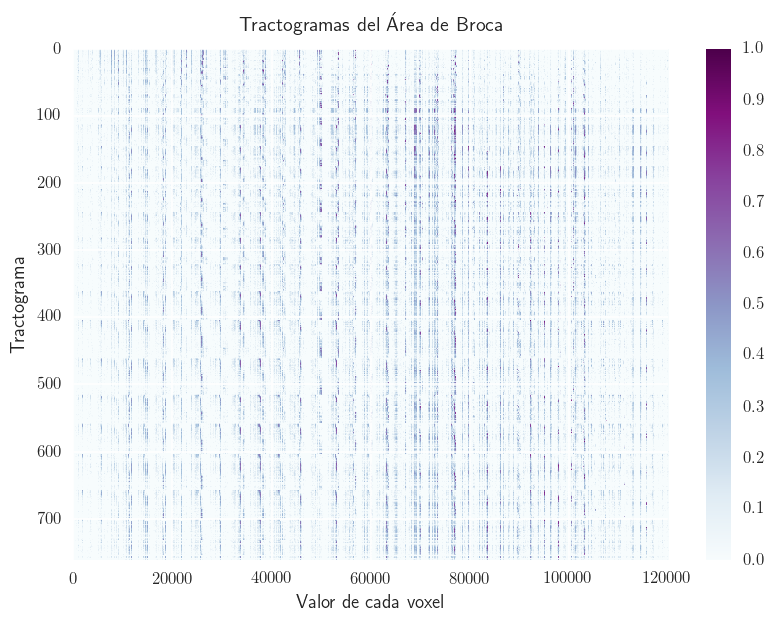
\includegraphics[width=0.9\textwidth]{img/densa_broca.png}
    \caption{Semillas en el hemisferio izquierdo. }
    \label{fig:densa}
\end{figure}

El problema de este \'ultimo m\'etodo es que a\'un desperdicia mucho espacio. En
el caso de utilizar todas los \textbf{tractogramas sin transformar} de un 
hemisferio, la matriz pasa a ser de dimensiones $21657\times3587328$ con un $1\%$
de valores no nulos. Para almacenar dicha matriz es necesario utilizar $587$ 
Gigabytes. Por esto es necesario utilizar estructuras mas eficiente, que aprovechen
lo ralo de las matrices. Ejemplos de estas estructuras son: \textit{Dictionary of
Keys}, o una matriz \textit{Compressed Sparse Row} (CSR). \\

%eliminando columnas in\'utiles nos queda 21657x145574, son 23.5 Gn

Si recordamos la forma que tiene la funci\'on logit encontramos un inconveniente
al querer utilizar matrices ralas. Podemos ver en la Figura \ref{fig:dominio} que
\textit{logit}$(0) = -\infty$. Esto implica que la transformaci\'on de una matriz
rala no es rala en t\'erminos de elementos nulos. Sin embargo podemos aprovechar
ciertas propiedades para recuperar las matrices ralas. La distancia euclidena 
entre vectores es invariante a traslaciones lineales del sistema. Lo mismo sucede
con las posiciones relativas de los centroides. Asignemos una representaci\'on 
finita $c$ al valor $-\infty$. Un buen candidato para $c$ es el $log(\epsilon)$,
donde $\epsilon$ es el \textit{epsilon de la maquina}. Transformar todos los vectores
y luego trasladarlos sumando $c$ en cada componente dara como resultado una
representaci\'on rala. Gracias a esto podemos utilizar DOK, CSR o cualquier
estructura para reducir los costos espaciales del clustering. \\








\blankpage


\chapter{Resultados}
\label{ch:resultados}

En el capitulo \ref{ch:metodos} presentamos la t\'ecnica de 
\textit{bootstraping}; el m\'etodo de Moreno-Dominguez para agrupar
tractogramas junto con algunas de sus falencias te\'oricas y como
solucionarlas usando la funci\'on \textit{logit}. En la secci\'on 
\ref{ch:nuestro}, presentamos nuestro m\'etodo para parcelar la corteza en
su totalidad. En las siguientes secciones mostramos primero los resultados
obtenidos al estudiar la estabilidad de los tractogramas; luego parcelamos
el \'area de Broca con ambos m\'etodos y finalmente parcelamos el
hemisferio derecho usando tambi\'en ambos m\'etodos. Todos los estudios se
realizaron sobre una misma mujer diestra de entre 23 y 26 a\~nos. Sus datos
fueron descargados de la base de datos \textit{Human Connectome Project}
\cite{VanEssen2012}. \\


\section{Estabilidad tractogramas}

Las Figuras \ref{fig:m1}, \ref{fig:m2} y \ref{fig:m3} muestran, para tres semillas
distintas, cinco cortes axiales del tractograma que se consigue al utilizar quince
mil part\'iculas.\\

Las Figuras \ref{fig:s1}, \ref{fig:s2} y \ref{fig:s3} muestran la varianza de 
cada voxel dentro de un mismo corte axial. La varianza se calcul\'o generando
mil tractogramas desde distinto n\'umero de streamlines. \\

La Figura \ref{fig:mv} muestra la media y varianza de los voxels $A$, $B$ y $C$
marcados en las Figuras \ref{fig:s1}, \ref{fig:s2} y \ref{fig:s3}. Estos voxels
fueron los que mayor varianza presentaron al generar tractogramas con dos mil
\textit{streamlines}.


\begin{figure}[h!]
   \centering
    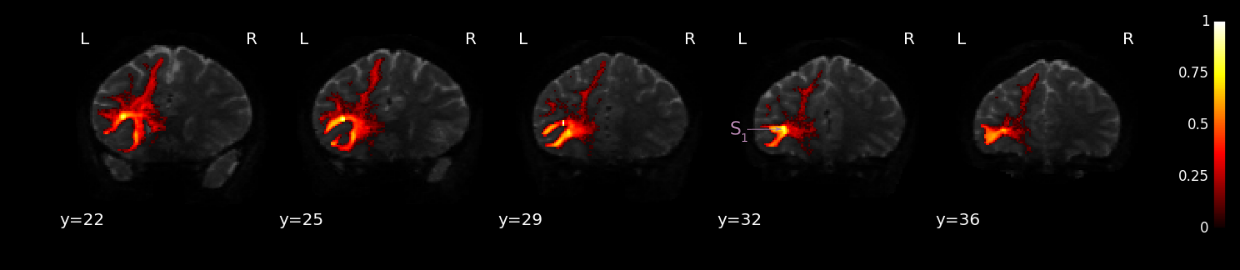
\includegraphics[width=\textwidth]{img/m1.png}
    \caption{Tractograma para la semilla $S1$ utilizando toda la muestra.}
    \label{fig:m1}
\end{figure}

\begin{figure}[h!]
   \centering
    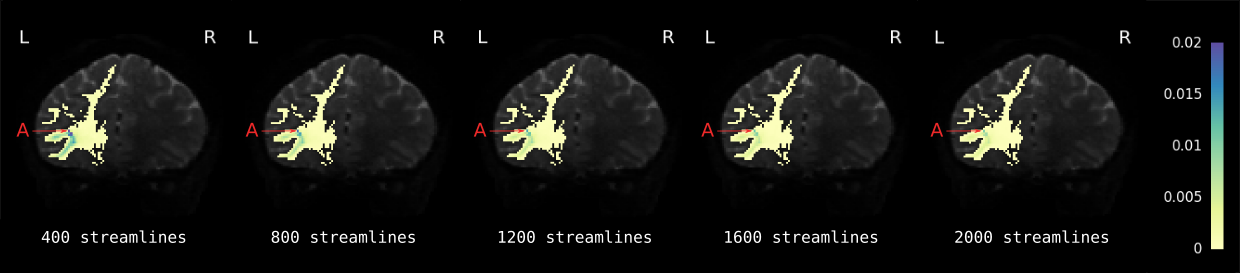
\includegraphics[width=\textwidth]{img/s1.png}
    \caption{Desviaci\'on Estandar respecto a la semilla $S1$. Mismo corte axial
             variando el tama\~no de las submuestras.}
    \label{fig:s1}
\end{figure}

\begin{figure}[h!]
   \centering
    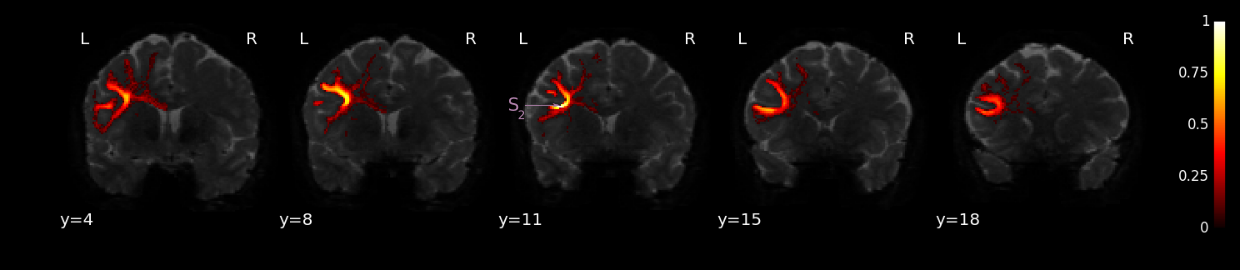
\includegraphics[width=\textwidth]{img/m2.png}
    \caption{Tractograma para la semilla $S2$ utilizando toda la muestra.}
    \label{fig:m2}
\end{figure}

\begin{figure}[h!]
   \centering
    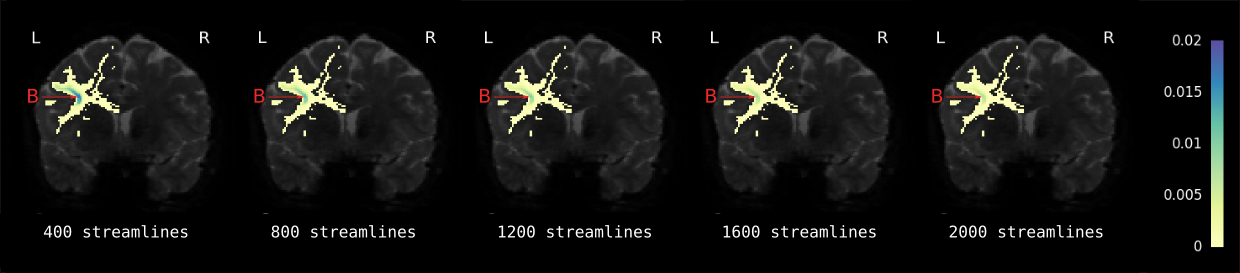
\includegraphics[width=\textwidth]{img/s2.png}
    \caption{Desviaci\'on Estandar respecto a la semilla $S2$. Mismo corte axial
             variando el tama\~no de las submuestras.}
    \label{fig:s2}
\end{figure}

\begin{figure}[h!]
   \centering
    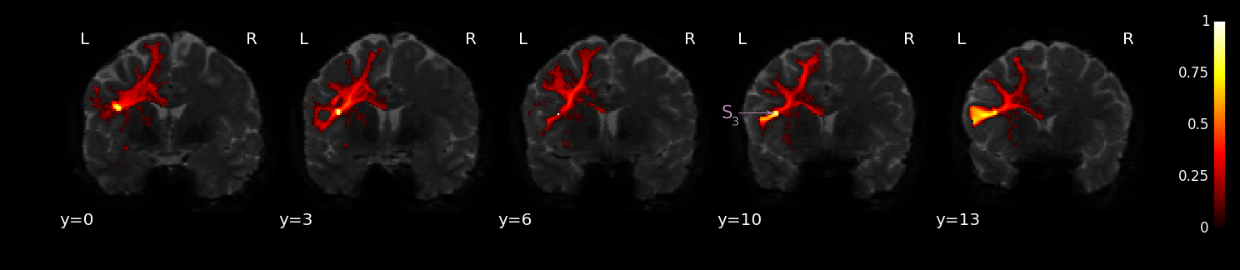
\includegraphics[width=\textwidth]{img/m3.png}
    \caption{Tractograma para la semilla $S3$ utilizando toda la muestra}
    \label{fig:m3}
\end{figure}

\begin{figure}[h!]
   \centering
    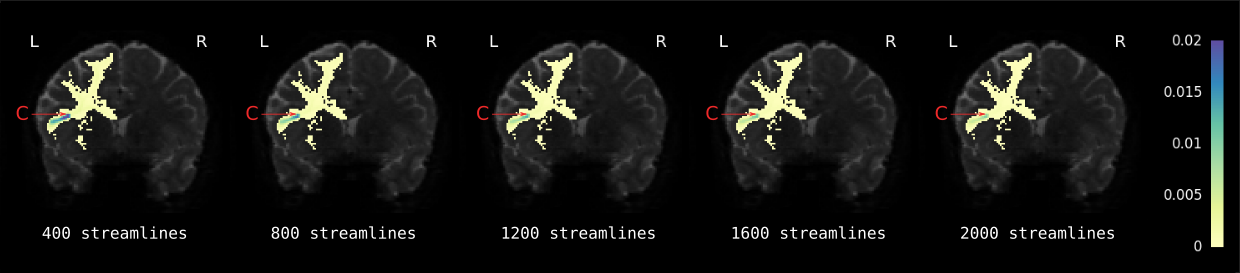
\includegraphics[width=\textwidth]{img/s3.png}
    \caption{Desviaci\'on Estandar respecto a la semilla $S3$. Mismo corte axial
             variando el tama\~no de las submuestras.}
    \label{fig:s3}
\end{figure}

\begin{figure}[h!]
   \centering
    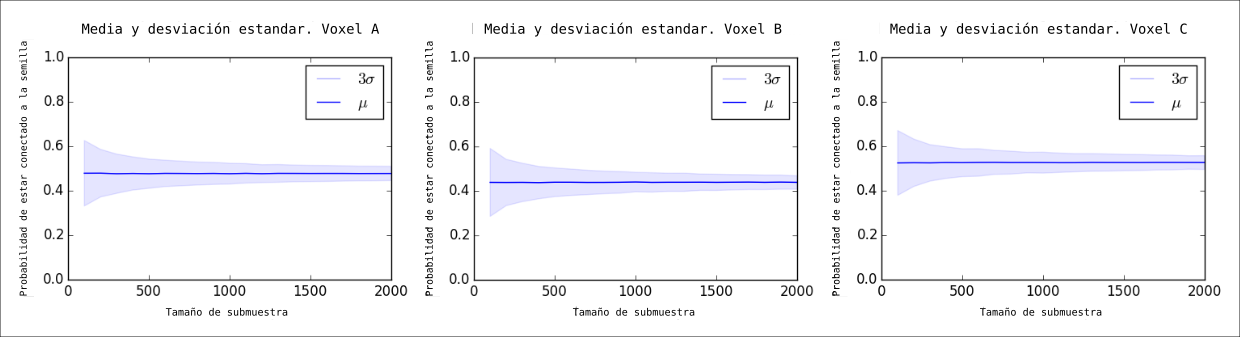
\includegraphics[width=\textwidth]{img/med_var_all.png}
    \caption{Media y desviaci\'on estandar de los voxels con mayor varianza.}
    \label{fig:mv}
\end{figure}


\section{Parcelando el \'Area de Broca}

\subsection{Distancia coseno con centroide}

Las siguientes Figuras muestran los resultados obtenidos al parcelar el \'Area
de Broca utilizando el m\'etodo de Moreno-Dominguez.

\begin{figure}[h!]
                                                                                                                        
\begin{minipage}[b]{\textwidth}
    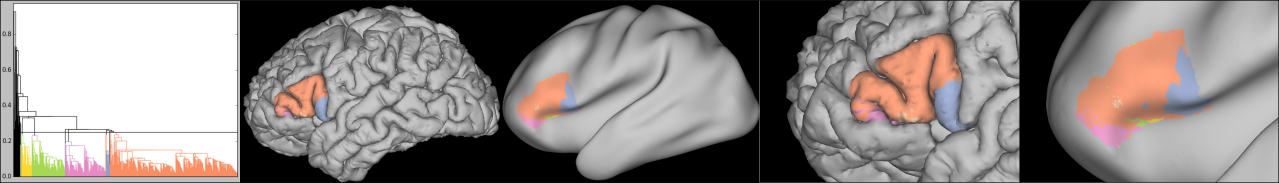
\includegraphics[width=\textwidth]{img/broca/moreno_0.png}
    \caption{M\'etodo Moreno sin preprocesamiento}

\end{minipage} ~
                                                                                                                       
\begin{minipage}[b]{\textwidth}
    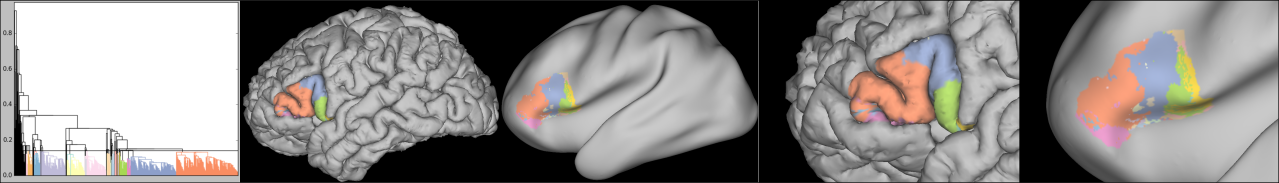
\includegraphics[width=\textwidth]{img/broca/moreno_0_deep.png}
    \caption{M\'etodo Moreno sin preprocesamiento, mayor profundidad en el 
            dendrograma}

\end{minipage} ~

\begin{minipage}[b]{\textwidth}
    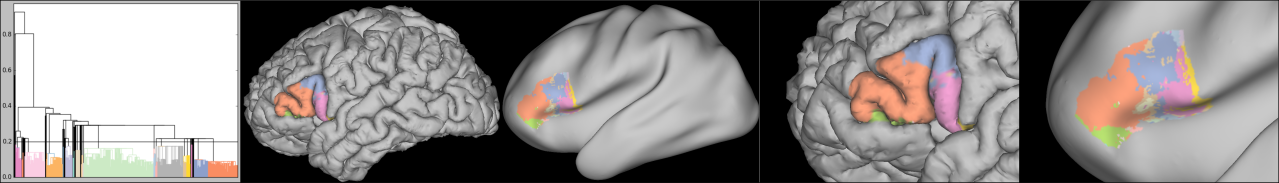
\includegraphics[width=\textwidth]{img/broca/moreno_400.png}
    \caption{M\'etodo Moreno, cuatrocientos pasos de preprocesamiento}

\end{minipage} ~

\begin{minipage}[b]{\textwidth}
    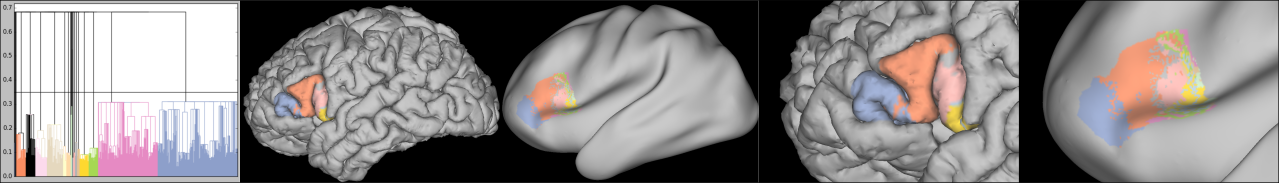
\includegraphics[width=\textwidth]{img/broca/moreno_750.png}
    \caption{M\'etodo Moreno, setecientos pasos de preprocesamiento}

\end{minipage} ~

\end{figure} 


\subsection{Utilizando LogOdds}

Las siguientes Figuras muestran los resultados obtenidos al parcelar el \'Area
de Broca utilizando el m\'etodo de Moreno-Dominguez. El threshold utilizado fue
de $0.25$. \textbf{Los resultados obtenidos luego de normalizar los vectores 
fueron tan malos que no vale la pena incluirlos}.

\begin{figure}[h!]
                                                                                                                        
\begin{minipage}[b]{\textwidth}
    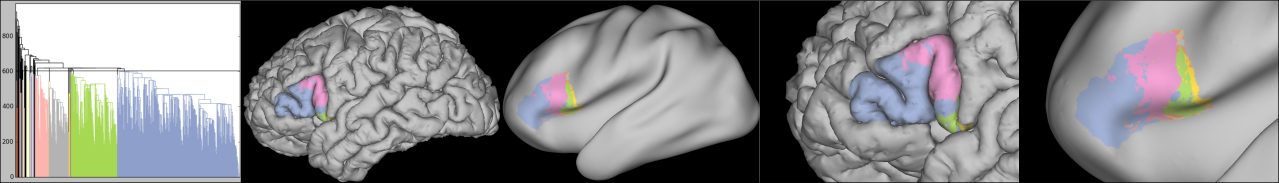
\includegraphics[width=\textwidth]{img/broca/logit_0.png}
    \caption{M\'etodo Logit sin preprocesamiento}
    \label{fig:dmri}
\end{minipage} ~
                                                                                                                        
\begin{minipage}[b]{\textwidth}
    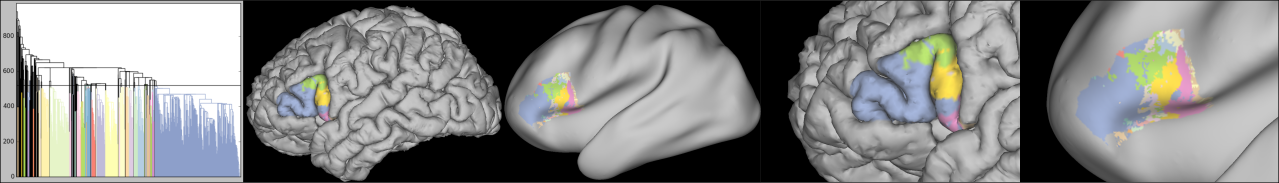
\includegraphics[width=\textwidth]{img/broca/logit_0_deep.png}
    \caption{M\'etodo Logit sin preprocesamiento, mayor profundidad en el 
            dendrograma}

\end{minipage} ~

\begin{minipage}[b]{\textwidth}
    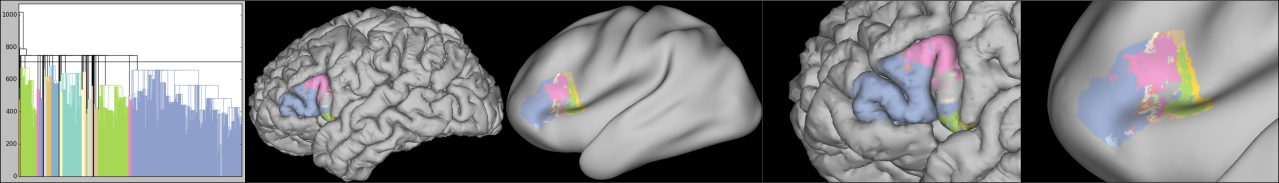
\includegraphics[width=\textwidth]{img/broca/logit_400.png}
    \caption{M\'etodo Logit, cuatrocientos pasos de preprocesamiento}

\end{minipage} ~

\begin{minipage}[b]{\textwidth}
    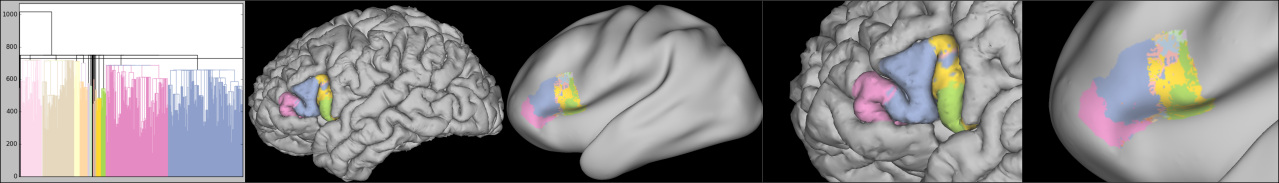
\includegraphics[width=\textwidth]{img/broca/logit_750.png}
    \caption{M\'etodo Logit, setecientos pasos de preprocesamiento}

\end{minipage} ~

\end{figure}


\subsection{Lado a lado}


\begin{figure}[h]

\begin{minipage}[h]{\textwidth}
    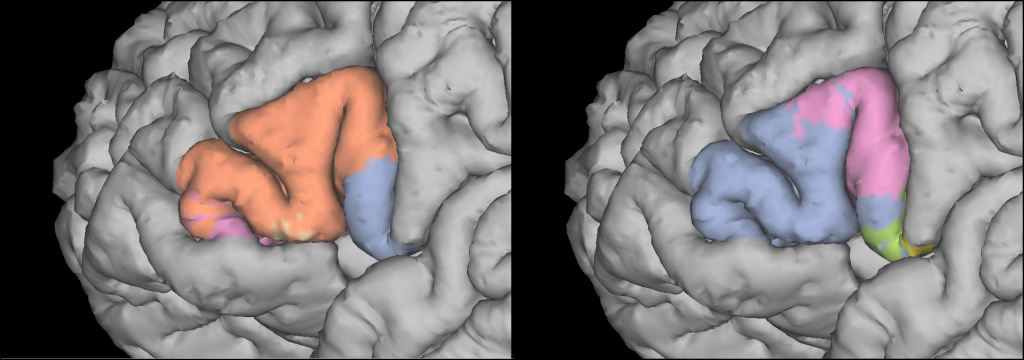
\includegraphics[width=\textwidth]{img/broca/vs_0.png}
    \caption{M\'etodo Moreno (izquierda) y Logit (derecha) sin preprocesamiento}
\end{minipage} ~

\end{figure}

\begin{figure}[h]                  

\begin{minipage}[h]{\textwidth}
    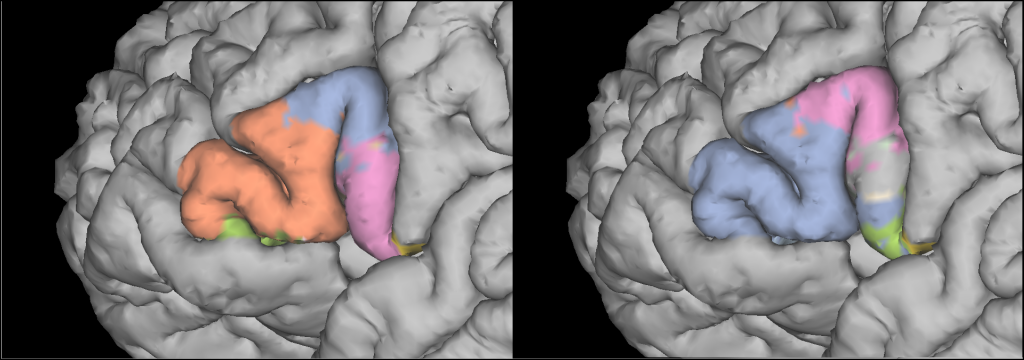
\includegraphics[width=\textwidth]{img/broca/vs_400.png}
    \caption{M\'etodo Moreno (izquierda) y Logit (derecha). Cuatrocientos pasos de preprocesamiento}
\end{minipage} ~

\end{figure}

\begin{figure}[h]

\begin{minipage}[h]{\textwidth}
    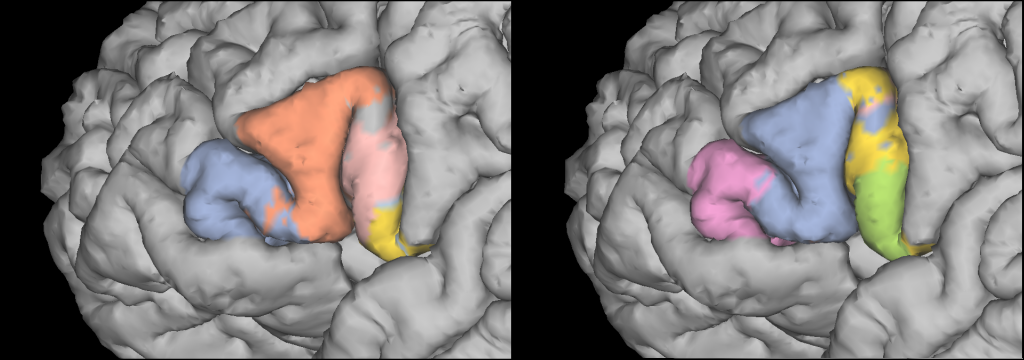
\includegraphics[width=\textwidth]{img/broca/vs_700.png}
    \caption{M\'etodo Moreno (izquierda) y Logit (derecha). Setecientos pasos de preprocesamiento}

\end{minipage} ~

\end{figure}
 


\section{Parcelando la corteza}

\subsection{Utilizando LogOdds}

\begin{figure}[h!]
                                                                                                                        
\begin{minipage}[b]{\textwidth}
    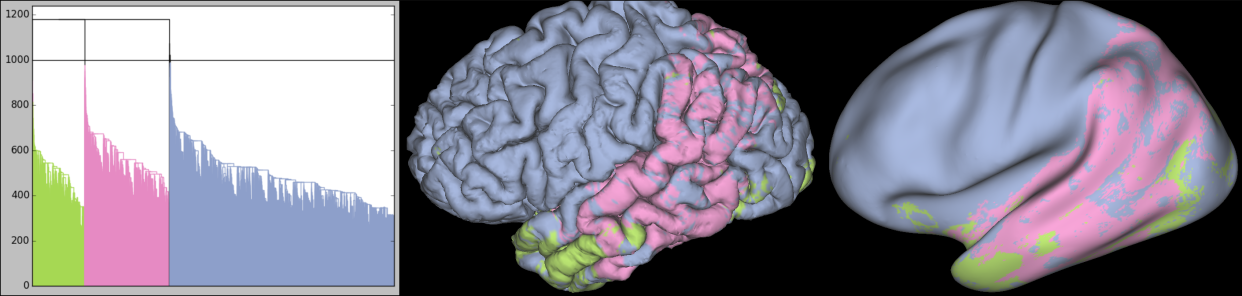
\includegraphics[width=\textwidth]{img/all_brain/logit_0.png}
    \caption{M\'etodo Logit sin preprocesamiento}
    \label{fig:dmri}
\end{minipage} ~
                                                                                                                        
\begin{minipage}[b]{\textwidth}
    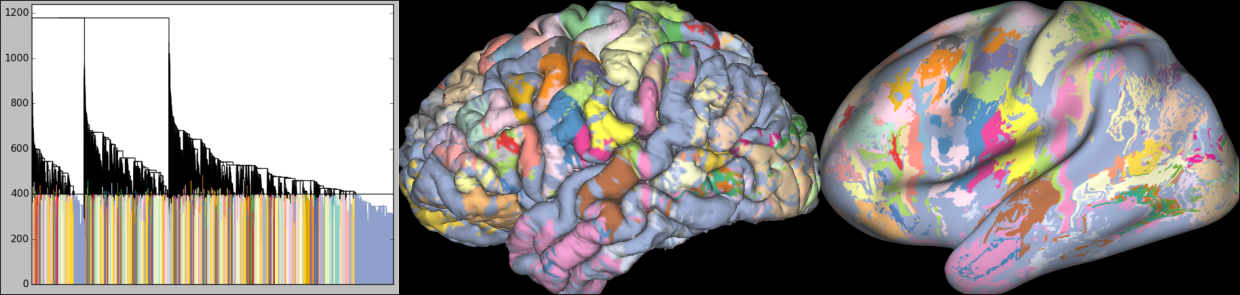
\includegraphics[width=\textwidth]{img/all_brain/logit_0_deep.png}
    \caption{M\'etodo Logit sin preprocesamiento, mayor profundidad en el 
            dendrograma}

\end{minipage} ~

\begin{minipage}[b]{\textwidth}
    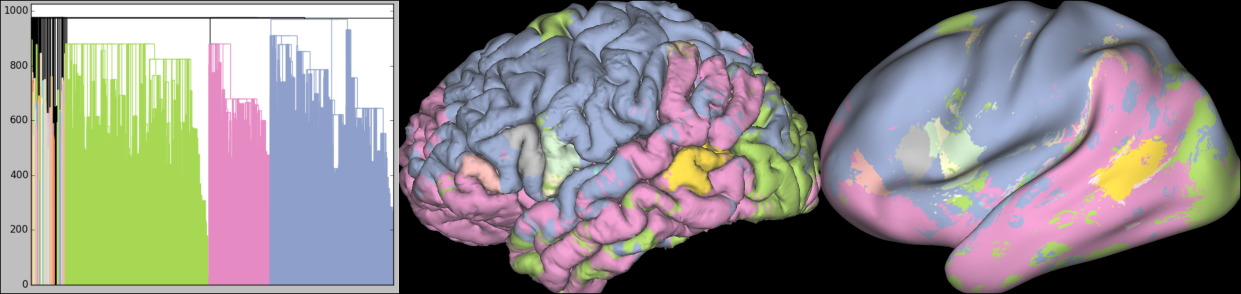
\includegraphics[width=\textwidth]{img/all_brain/logit_20000.png}
    \caption{M\'etodo Logit, veinte mil pasos de preprocesamiento}

\end{minipage} ~

\begin{minipage}[b]{\textwidth}
    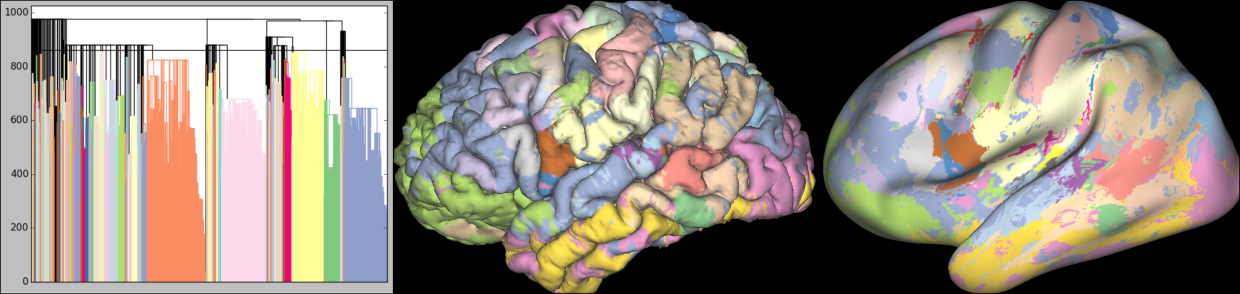
\includegraphics[width=\textwidth]{img/all_brain/logit_20000_deep0.png}
    \caption{M\'etodo Logit, veinte mil pasos de preprocesamiento, mayor 
             profundidad}
\end{minipage} ~

\begin{minipage}[b]{\textwidth}
    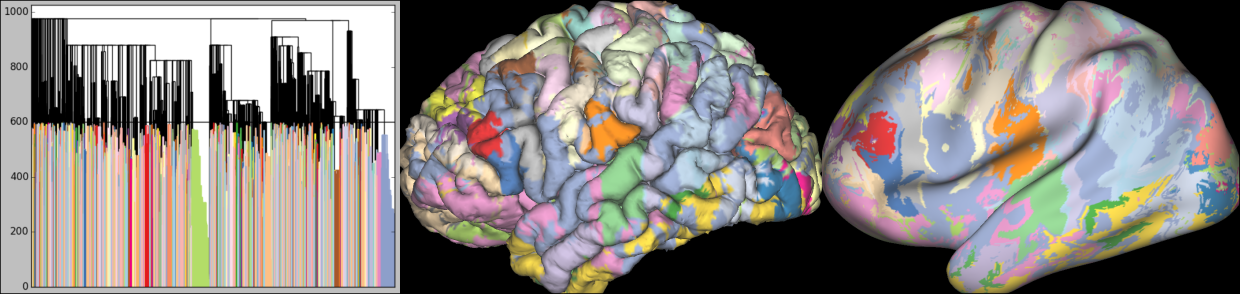
\includegraphics[width=\textwidth]{img/all_brain/logit_20000_deep1.png}
    \caption{M\'etodo Logit, veinte mil pasos de preprocesamiento, mayor 
             profundidad}
\end{minipage} ~


\end{figure}



\chapter{Discusi\'on} 

Como explicamos al principio de este trabajo, existe evidencia de que es posible
parcelar el cerebro mediante un criterio funcional. Esto es, dividir el cerebro
en distintas regiones, atribuyendo una funci\'on a cada una de ellas \cite{Greicius2003}.
A su vez, la Resonancia Magn\'etica de Difusi\'on ha permitido desarrollar nuevos 
criterios estructurales de parcelaci\'on \cite{Taylor1985}. A lo largo de este
trabajo nos enfocamos en estudiar el reciente aporte de Moreno-Dominguez 
\cite{Moreno-Dominguez2014}. El mismo se basa en utilizar un algoritmo de
tractograf\'ia y otro de \textit{clustering} para parcelar la corteza cerebral. 
Luego, basandonos en su trabajo, propusimos un nuevo algoritmo de \textit{clustering},
tambi\'en basado en tractograf\'ias. En este \'ultimo capitulo discutiremos los 
resultados obtenidos. Comenzando por la robustes del algoritmo de tractograf\'ia
utilizado; siguiendo con una comparaci\'on entre nuestro m\'etodo y el de 
Moreno-Dominguez; luego hablaremos sobre la validez biol\'ogica de la parcelaci\'on
obtenida y propondremos objetos de futuro estudio. \\


\section{Convergencia del algoritmo de tractograf\'ia}

El algoritmo utilizado en el trabajo demostr\'o ser estable. Las figuras 
\ref{fig:s1}, \ref{fig:s2} y \ref{fig:s3} muestran que la desviaci\'on estandar
es casi nula al usar quince mil part\'iculas. A su vez, la figura \ref{fig:mv}
muestra lo r\'apido que converge la media de tres voxels distintos. Como eran los 
de mayor desv\'io estandar, podemos asegurar que casi no existe diferencia en 
la media de los tractogramas creados con dos mil part\'iculas. Nuestro m\'etodo
se basa en tractogramas, por lo que es importante contar con un algoritmo de 
tractograf\'ia robusto.

\section{Comparaci\'on entra ambos m\'etodos}

En ambos casos sucedi\'o que a mayor n\'umero $k$, menos dispersas quedaron las
distintas parcelas. Recordemos que $k$ es la cantidad de uniones que se har\'an
solo entre clusters vecinos. Respecto a las \'areas obtenidas, en la divisi\'on
del \'area de Broca los resultados fueron similares. La secci\'on \ref{sec:acercamiento} 
permite ver esto de manera explicita. Sin embargo, al pasar a la parcelaci\'on 
del hemisferio completo resulta dif\'icil realizar una simple comparaci\'on visual.
M\'as a\'un, es complicado encontrar cortes en los dendrogramas que generen 
representaciones parecidas. Sin embargo, en la secci\'on \ref{sec:acercamiento_corteza}
se puede ver que ambos resultados comparten similitudes. Por ejemplo, las 
siguientes estructuras son parecidas: la corteza motora y la somest\'esica; 
el lobulo frontal y occipital, as\'i como tambi\'en el \'area de Broca.


\section{Validaci\'on anat\'omica y funcional}

Dada la dificultad de comparar nuestro m\'etodo visualmente con el de Moreno-Dominguez
buscamos otra forma de validarlo. En la figura \ref{fig:an2pa} se puede ver
el resultado de proyectar la parcelaci\'on anat\'omica del sujeto sobre la que
obtuvimos. En interesante notar como nuestra parcelaci\'on cre\'o \'areas dentro
de los l\'imites de al menos 9 regiones an\'atomicas. En particular, la divisi\'on
del \'area motora parece ser consistente con la literatura actual. Por ello 
tambi\'en comparamos la parcelaci\'on con un estudio funcional hecho sobre el 
sujeto \cite{Barch2013}. 

\begin{figure}[h!]
    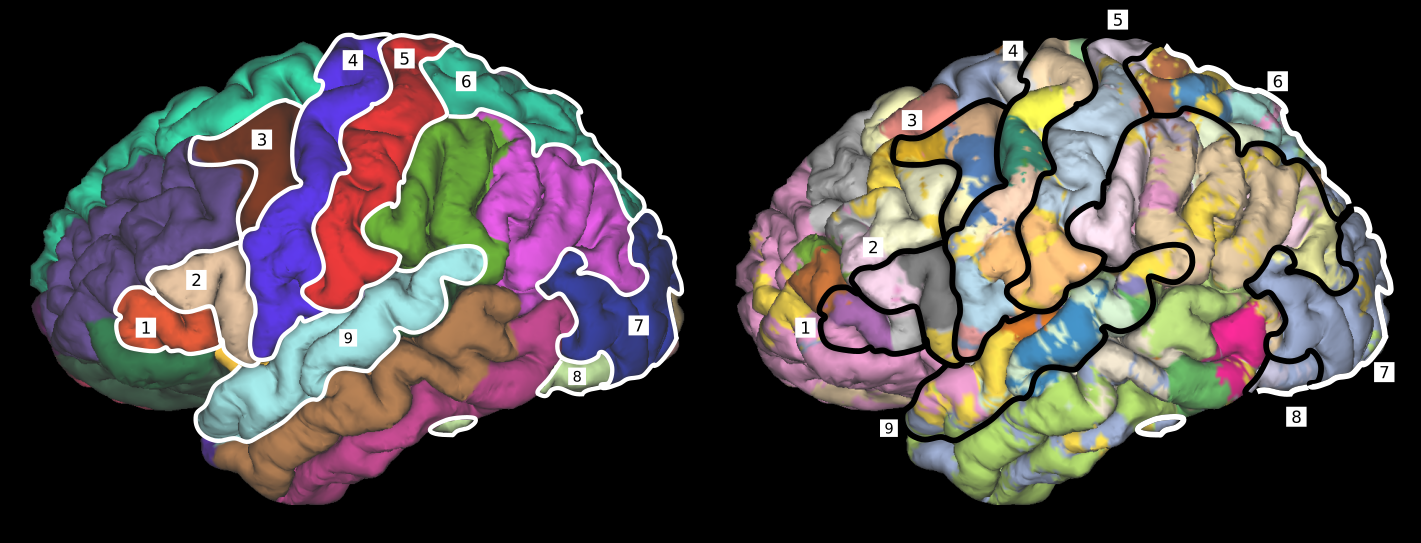
\includegraphics[width=\textwidth]{img/anatomica2parcelation.png}
    \caption{Proyecci\'on del atlas anat\'omico (izquierda) a la parcelaci\'on obtenida (derecha)}
    \label{fig:an2pa}
\end{figure}

\begin{figure}[h!]
    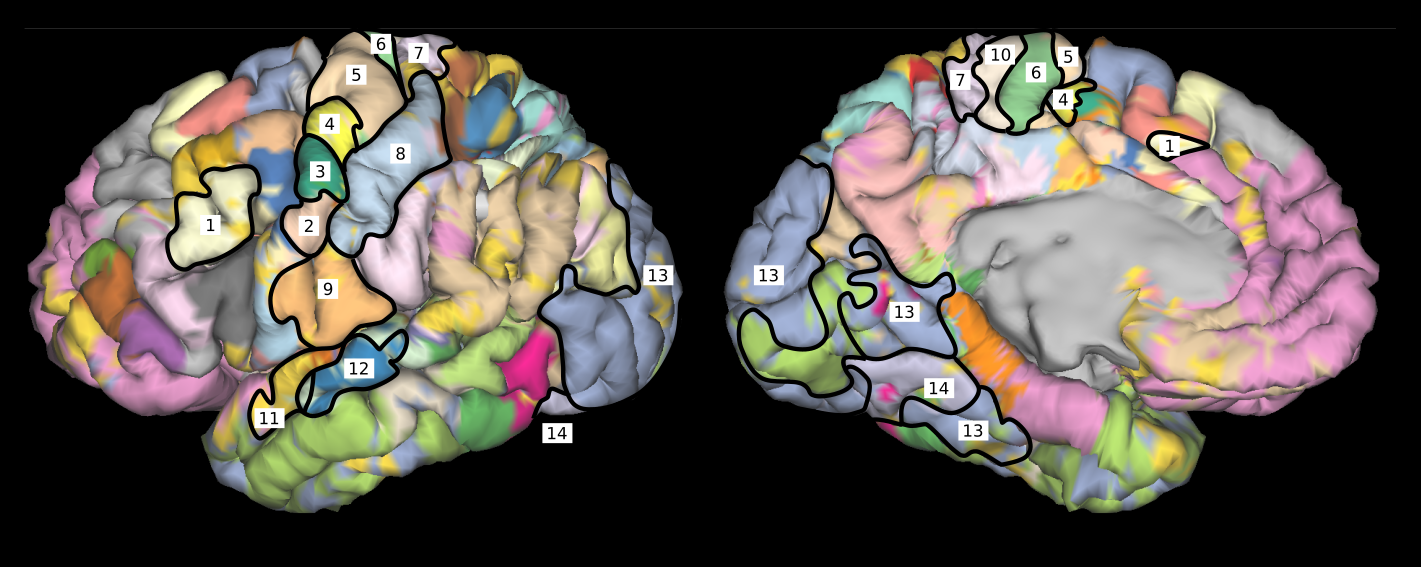
\includegraphics[width=\textwidth]{img/32k_labels.png}
    \caption{Parcelas en baja resoluci\'on}
    \label{fig:32k}
\end{figure}


\begin{figure}[h!]
    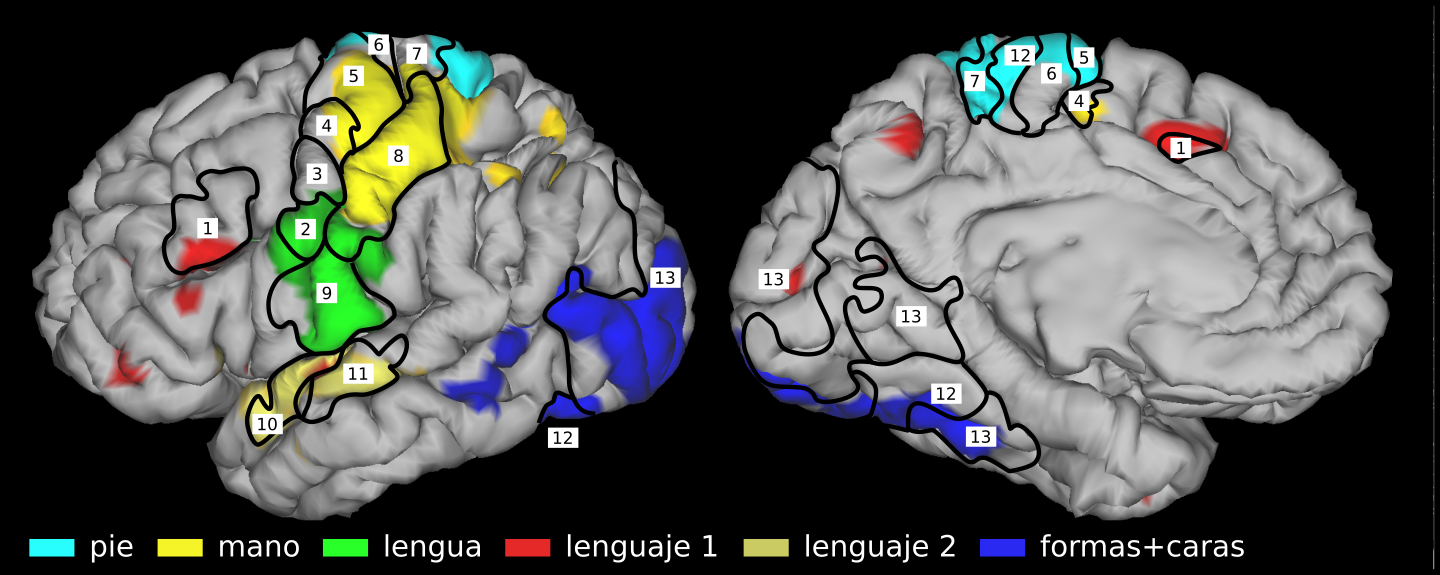
\includegraphics[width=\textwidth]{img/32k_z5.png}
    \caption{Projecci\'on de las parcelas (izquierda) sobre activaciones funcionales (derecha)}
    \label{fig:32k}
\end{figure}

\begin{figure}[h!]
    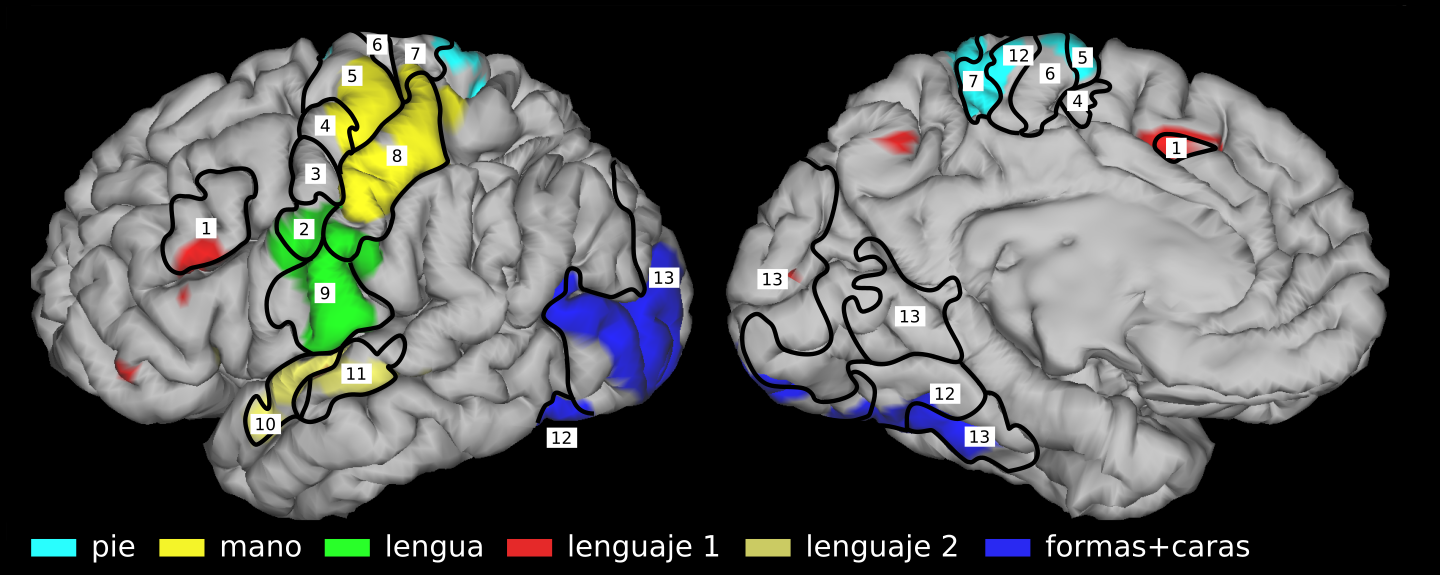
\includegraphics[width=\textwidth]{img/32k_z7.png}
    \caption{Projecci\'on de las parcelas (izquierda) sobre activaciones funcionales con 
             mayor valor de z-score (derecha)}
    \label{fig:32k}
\end{figure}


%%%% BIBLIOGRAFIA
\backmatter
%\begin{thebibliography}{9}

\bibitem{anwander07} Anwander, A., Tittgemeyer, M., von Cramon, D.Y., Friederici, A.D., Knösche, T.R., \emph{Connectivity-based parcellation of Broca's area.} \textit{Cereb Cortex} 17, 816-825. 2007. 

\bibitem{barch13} Barch, D. M., Burgess, G. C., Harms, M. P., Petersen, S. E., Schlaggar, B. L., Corbetta, M., et al. \emph{Function in the human connectome: Task-fMRI and individual differences in behavior.} \textit{Neuroimage} 80, 169–189. doi:10.1016/j.neuroimage.2013.05.033. 2013.

\bibitem{behrens03} Behrens, Johansen-Berg, Woolrich,  Smith, Wheeler-Kingshott, Barker, Sillery, Sheehan, Ciccarelli, Thompson, Brady, Matthews, \emph{No n-invasive mapping of connections between human thalamus and cortex using diffusion imaging}. \textit{Nat Neurosci} 6, 750-757. 2003.

\bibitem{brodman09} Brodmann,  K., \emph{Vergleichende  Lokalisationslehre  der  Großhirnrinde  in ihren Prinzipien dargestellt auf Grund des Zellaufbaues}. Barth, Leipzig. 1909. 

\bibitem{callaghan91} Callaghan P. T. , A. Coy, D. MacGowan, K. J. Packer, F. O. Zelaya. \emph{Diffraction-like effects in NMR diffusion studies of fluids in porous solids} \textit{Nature}; 351(6326):467-469. 1991.

\bibitem{descoteaux09} Descoteaux, M., Deriche, R., Knösche, T., \& Anwander, A. (2009). \emph{Deterministic and Probabilistic Tractography Based on Complex Fiber Orientation Distributions}. \textit{IEEE Transactions on Medical Imaging}, 28(2), 269–286.

\bibitem{greicius02} Michael D. Greicius, Ben Krasnow, Allan L. Reiss and Vinod Menon. \emph{Functional connectivity in the resting brain: A network analysis of the default mode hypothesis}. Washington University School of Medicine. 2002.

\bibitem{hartigan79} Hartigan, J. A.; Wong, M. A. \emph{Algorithm AS 136: A K-Means Clustering Algorithm}. \textit{Journal of the Royal Statistical Society, Series C} 28 (1): 100–108. JSTOR 2346830. 1979.

\bibitem{hastie09} Hastie, Trevor; Tibshirani, Robert; Friedman, Jerome. \emph{The Elements of Statistical Learning}. New York: Springer. pp. 236-243. ISBN 0-387-84857-6. 2009.

\bibitem{hastie09b} Hastie, Trevor; Tibshirani, Robert; Friedman, Jerome. \emph{The Elements of Statistical Learning}. New York: Springer. pp. 520–528. ISBN 0-387-84857-6. 2009.

\bibitem{jbabdi14} Jbabdi, S., Woolrich, M. W., Andersson, J. L. R., \& Behrens, T. E. J. (2007). \emph{A Bayesian framework for global tractography.}, \textit{NeuroImage}, 37(1), 116–129. doi:10.1016/j.neuroimage.2007.04.039.

\bibitem{moreno14} Moreno-Dominguez D., Anwander A, Knösche TR \emph{A hierarchical method for whole-brain connectivity-based parcellation.}, \textit{Hum Brain Mapp}, 35(10):5000-25. doi: 10.1002/hbm.22528. Epub 2014.

\bibitem{pohl07} Pohl KM1, Fisher J, Bouix S, Shenton M, McCarley RW, Grimson WE, Kikinis R, Wells WM. \emph{Using the logarithm of odds to define a vector space on probabilistic atlases}. \textit{Med Image Anal}. 11(5):465-77. 2007.

\bibitem{stejskal65} Stejskal, E. O.; Tanner, J. E. \emph{Spin Diffusion Measurements: Spin Echoes in the Presence of a Time-Dependent Field Gradient}. \textit{The Journal of Chemical Physics} 42 (1): 288. 1965

\bibitem{tournier04} Tournier, J.D., Calamante, F., Gadian, D.G., Connelly, A., \emph{Direct estimation of the fiber orientation density function from diffusion-weighted MRI data using spherical deconvolution.} \textit{Neuroimage} 23, 1176–1185. 2004.

\bibitem{tuch04} Tuch D. S., \emph{Q-ball  imaging} \textit{Magn. Reson. Med.} ;52;6, 1358–1372. 2004.

\bibitem{Lipton2014} Michael L. Lipton [Albert Einstein College of Medicine]. Introducing MRI [Video file]. Retrieved from https://www.youtube.com/watch?v=35gfOtjRcic. 2014. 




\end{thebibliography}



\bibliographystyle{ieeetr}
\bibliography{bibtex}

\end{document}
